\documentclass[]{spie}  %>>> use for US letter paper
%\documentclass[a4paper]{spie}  %>>> use this instead for A4 paper
%\documentclass[nocompress]{spie}  %>>> to avoid compression of citations

\renewcommand{\baselinestretch}{1.0} % Change to 1.65 for double spacing
 
\usepackage{amsmath,amsfonts,amssymb}
\usepackage{graphicx}
\usepackage[colorlinks=true, allcolors=blue]{hyperref}
\usepackage{subfigure}

\title{Pulmonary lobar segmentation from computed tomography scans based on a statistical finite element analysis of lobe shape}

\author[1]{Yuwen Zhang}
\author[1]{Mahyar Osanlouy}
\author[1]{Alys R. Clark}
\author[1]{Hari Kumar}
\author[2]{Margaret L. Wilsher}
\author[2]{David G. Milne}
\author[3]{Eric A. Hoffman}
\author[1]{Merryn H. Tawhai}
\affil[1]{Auckland Bioengineering Institute, University of Auckland, Auckland, New Zealand}
\affil[2]{Auckland City Hospital, Auckland District Health Board, Auckland, New Zealand}
\affil[3]{Department of Radiology and Biomedical Engineering, University of Iowa, Iowa City, IA, USA}

%\authorinfo{Further author information: (Send correspondence to A.A.A.)\\A.A.A.: E-mail: aaa@tbk2.edu, Telephone: 1 505 123 1234\\  B.B.A.: E-mail: bba@cmp.com, Telephone: +33 (0)1 98 76 54 32}

% Option to view page numbers
\pagestyle{empty} % change to \pagestyle{plain} for page numbers   
\setcounter{page}{301} % Set start page numbering at e.g. 301
 
\begin{document} 
\maketitle

\begin{abstract}
Automatic identification of pulmonary lobes from imaging is important in disease assessment and treatment planning. However, the lobar fissures can be difficult to detect automatically, as they are thin, usually of fuzzy appearance and incomplete on CT scans. The fissures can also be obscured by or confused with features of disease, for example the tissue abnormalities that characterise fibrosis. Traditional anatomical knowledge-based methods rely heavily on anatomic knowledge and largely ignore individual variability, which may result in failure to segment pathological lungs. In this study, we aim to overcome difficulties in identifying pulmonary fissures by using a statistical finite element shape model of lobes to guide lobar segmentation. By deforming a principle component analysis based statistical shape model onto an individual’s lung shape, we predict the likely region of fissure locations, to initialize the search region for fissures. Then, an eigenvalue of Hessian matrix analysis and a connected component eigenvector based analysis are used to determine a set of fissure-like candidate points. A smooth multi-level $\beta$-spline curve is fitted to the most fissure-like points (those with high fissure probability) and the fitted fissure plane is extrapolated to the lung boundaries. The method was tested on 20 inspiratory and expiratory CT scans, and the results show that the algorithm performs well both in healthy young subjects and older subjects with fibrosis. The method was able to estimate the fissure location in 100\% of cases, whereas two comparison segmentation softwares that use anatomy-based methods were unable to segment 7/20 and 9/20 subjects, respectively. 
\end{abstract}

% Include a list of keywords after the abstract 
\keywords{pulmonary lobar segmentation, Statistical shape model, principal component analysis, Hessian matrix, CT}

\section{INTRODUCTION}
\label{sec:intro}  % \label{} allows reference to this section

Human lungs are divided into five lobes which form distinct anatomical regions separated by fissures. Identification of these lobes in imaging is important for assessment of lung disease severity and treatment planning. The lobes act somewhat independently of each other with respect to respiratory function, thus many pulmonary diseases act at a lobar level\cite{ukil2009anatomy}. For example, emphysema \cite{jeffery1998structural}, postprimary tuberculosis \cite{leung1999pulmonary} and silicosis \cite{rees2007silica} usually affect the upper lobes, while idiopathic pulmonary fibrosis commonly presents in the lower lobes \cite{lin2015combined}. For clinical applications, identification of the pulmonary fissures can be an important step in the image-based study of lung function and disease: knowing the lobar distribution of pulmonary disease is beneficial for doctors to recognize pathogenesis and guide therapy (including surgical planning)\cite{van2010automatic}. Segmentation of lobes can also facilitate intra-patient image registration for localizing and tracking disease progression, since lobes are important structural landmarks \cite{lassen2011interactive}. However, the lobes are difficult to segment automatically as they can appear as faint or fuzzy lines in imaging, fissures can be incomplete on CT scans (even in healthy patients), and there is anatomical variation in lobe shape and size between individuals. This anatomical variation is usually associated with age, sex, height and body mass index (BMI)\cite{ross2010automatic, gulsun2006variability}. 

In a broad sense, existing algorithms that aim to automatically segment pulmonary lobes consist of two steps: lung segmentation and fissure detection. Lung segmentation methods are well-established and most results are typically reliable\cite{hu2001automatic, ukil2005smoothing, sun20063d, pu2008adaptive, wang2009automated, sun2012automated}. In contrast, automated fissure detection is challenging, and currently no method has yet been demonstrated to be robust and effective across a wide range of clinical imaging parameters and pathology experienced in clinical practice. One class of proposed fissure detection method (anatomical knowledge based analysis method) makes use of either local or global knowledge of lung anatomy, such as airway and vessel trees, to help with identifying fissures\cite{kuhnigk2005informatics, zhou2004automatic, saita2006algorithm, ukil2009anatomy, pu2009computational, lassen2010automatic, doel2012pulmonary, lassen2013automatic}. For example, there are typically no large vessels in the vicinity of lobar fissures, and the bronchi can be classified into five lobes using an edge detection method, so fissures should be located in the gaps between airway and vessel trees. These methods can be time consuming to execute as airways and blood vessels must be identified as an intermediate step. If the airways or vessels cannot be segmented – for example, due to tissue abnormalities or failure division of airway main branches, then these methods cannot complete the fissure segmentation. A second class of fissure detection method (shape based analysis method) makes use of gray-level information and shape information to detect the fissures \cite{wiemker2005unsupervised, van2008supervised, van2010automatic, ross2010automatic, kitasaka2006recognition, lassen2011interactive, doel2012pulmonary, lassen2013automatic, ross2013pulmonary}. Generally, lobar fissures can be regarded as bright planes crossing the pulmonary volume because of the higher density value of fissures compared to the surrounding tissues. Based on this information, several published methods use a local filtering algorithm to detect the voxels which lie on these planes, so that these detected voxel points can construct a continuous fissure surface. Moreover, some researches take advantage of both of these two methods, with combining anatomical information and gray-level information together for fissure detection\cite{ukil2009anatomy, doel2012pulmonary, lassen2013automatic}. However, all these methods often face problems when lobe fissures are blurry or incomplete. Currently, there are some papers providing algorithms to detect incomplete fissures, such as fast matching method\cite{ukil2009anatomy}, thin plate spline (TPS)\cite{ross2013pulmonary} and $\beta$-spine smooth curve\cite{doel2012pulmonary}, through finding optimal fissure surfaces within regions of interest (ROIs). A further challenge for all segmentation methods is identifying the fissures in thin-slice CT that has large spacing between slices, and recognising fissures for scans containing physiologic abnormalities.

In this paper, we present a statistical finite element shape model-guided method to segment pulmonary lobes from CT images. This new procedure does not depend on prior segmentation of anatomical structures (airway lobar classification) and has promising potential as a clinically useful semi-automatic lobe segmentation procedure. Unlike 'deep learning' methods, this approach requires relatively few subject images as a training set. Development of this method was motivated by the poor reliability of existing methods for a guaranteed estimate of fissure location, particularly in volumetric images of abnormalities, or when only thin-slice CT (non-volumetric images) are available.

\section{METHOD}

Here, an statistical shape model (SSM) guided method is presented to segment pulmonary lobes from CT images. A three-step approach is followed for the lobe segmentation (shown in Figure \ref{fig:WholeWorkflow}): in the first step, a threshold-based lung segmentation method defines the lung boundary; in the second step, an SSM is deformed to provide a ''search region'' for fissure locations; in the third step, fissures are located using a Hessian matrix protocol combined with connected component filters and a surface fitting algorithm. 

\begin{figure}[htbp]
  \centering 
  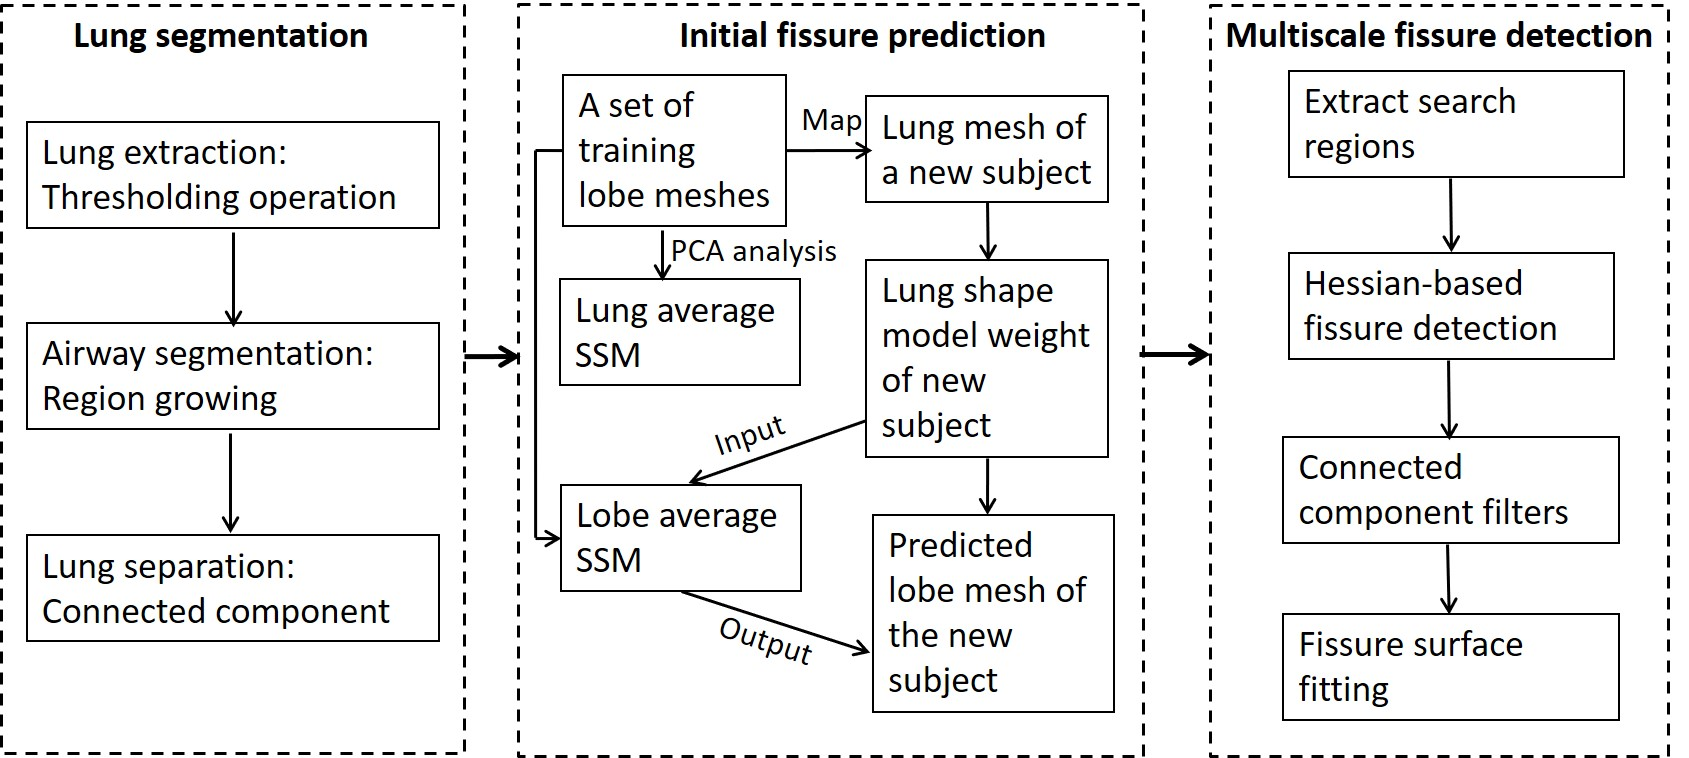
\includegraphics[height=2.7in]{Image/WholeWorkflow.jpg}
  \caption{Flow diagram of the lobar segmentation process.}
  \label{fig:WholeWorkflow}
\end{figure}

\subsection{Lung segmentation}
\label{LungSegmentation}

A good lung segmentation is a prerequisite for lobe segmentation, since all the other segmentations need to be performed inside the two lung regions. Here, a common thresholding method was used to segment the lungs \cite{ukil2005smoothing}. The procedure consists of the following steps: 1) uses a thresholding operation (-775 Hounsfield Units) and connected component identification to find the initial lung regions and trachea location, 2) by using the most apical point of the trachea as a starting point, a region growing technique is applied to detect the airway trees, and 3) left and right lungs are separated as the two largest connected components remaining after removing the trachea and main left and right bronchi. Figure \ref{fig:LungSegmentation} shows a typical lung segmentation result.

\begin{figure}[htbp] 
\centering
\begin{subfigure}{
  \begin{minipage}[t]{0.3\linewidth}
  \sbox0{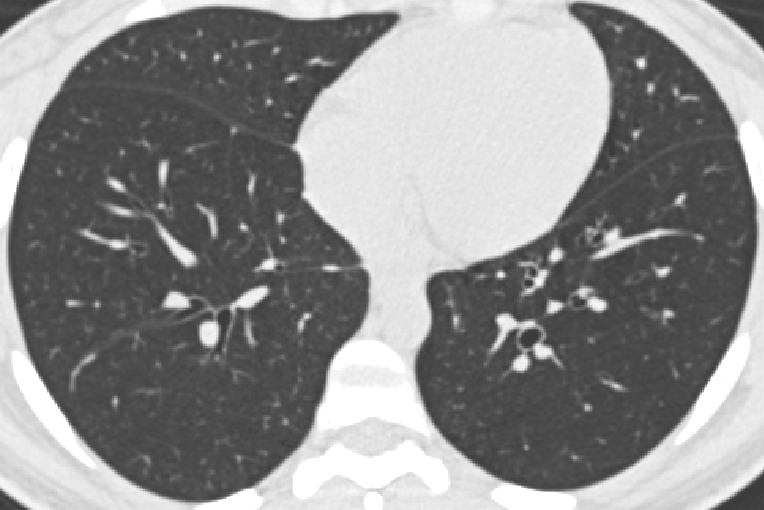
\includegraphics{Image/LungSegmentationBefore.png}}
  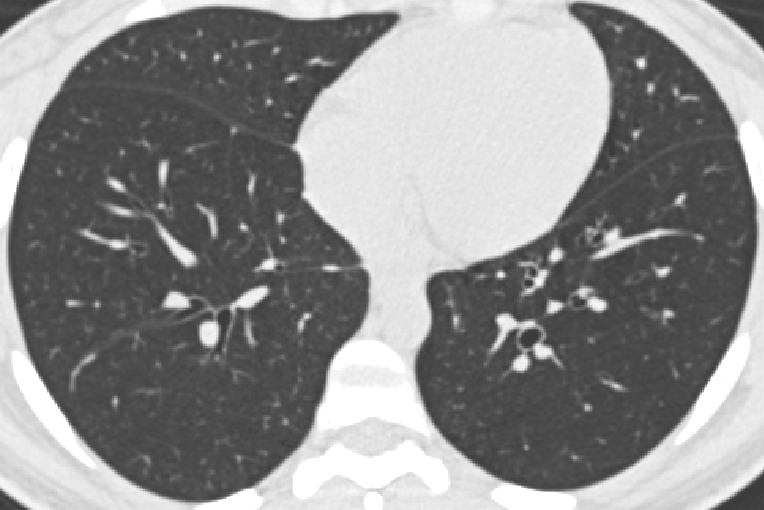
\includegraphics[width=\linewidth,trim={{.0\wd0} {.0\wd0} {.0\wd0} {.0\wd0}},clip]{Image/LungSegmentationBefore.png}
	\centerline{Before lung segmentation}
  \label{fig:LungSegmentation-a} 
	\end{minipage}%
   }%
\end{subfigure}
\begin{subfigure}{
  \begin{minipage}[t]{0.3\linewidth}
  \sbox0{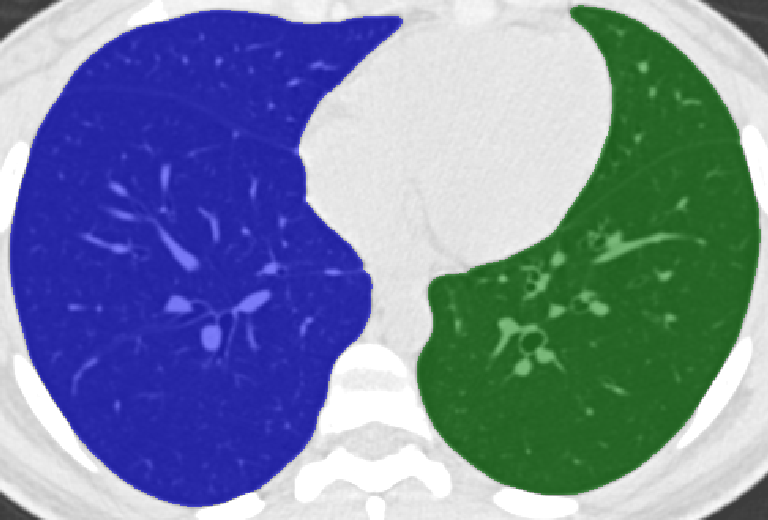
\includegraphics{Image/LungSegmentationAfter.png}}
  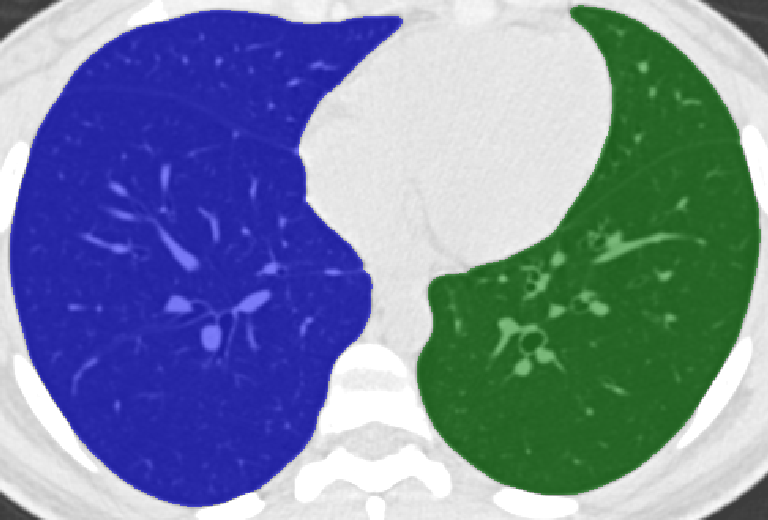
\includegraphics[width=\linewidth,trim={{.0\wd0} {.0\wd0} {.0\wd0} {.0\wd0}},clip]{Image/LungSegmentationAfter.png}
  \centerline{After lung segmentation}
  \label{fig:LungSegmentation-b} 
  \end{minipage}%
   }%
\end{subfigure}
\caption{Lung segmentation result using the common thresholding method.}
\label{fig:LungSegmentation}
\end{figure}

\subsection{Statistical finite element models of lung and fissure shape} \label{ShapeModelGeneration}
To guide a statistical shape model based segmentation, the first step is to generate a statistical lobar shape mesh using a set of training data. Here, we employ a Statistical Finite element analysis of Lobe (SFeaL) based on an active shape model (ASM) \cite{cootes1995active}. To do this, a training set of segmented lung and fissure surface locations was used to describe a cohort of adults with radiologically normal lungs. This approach employs a finite element shape mesh to specify pulmonary lobar shape which provides an efficient parameterized representation of lobar boundaries and makes shape constraints available during image analysis. The training set consisted of data from 50 subjects. 35 subjects were selected from a study of non-smoking healthy subjects, the Human Aging Cohort (AGING) study (approved by the Northern A Health and Health and Disability Ethics Committees (HDEC), Ministry of Health on 29 April 2013 through the HDEC-Full Review Pathway - ethics reference 13/NT/41), and a further 15 subjects were selected from a separate study of younger non-smoking healthy subjects, the Human Lung Atlas (HLA) (approved by the University of Iowa Institutional Review Board). To define the lung shape, volumetric CT images were segmented using the method described in Section \ref{LungSegmentation}. The segmented lung surface was then digitized into a set of data points as a 3D-space representation of lung shape. Fissure surface segmentation was performed manually using the open-source visualization software CMGUI (https://www.cmiss.org/cmgui) by an expert user, to provide a gold-standard definition of the fissure location for each subject in the training set. A high order (bi-cubic Hermite) finite element mesh template with the same mesh connectivity for each subject was geometry fitted to the lung and fissure surface data for each subject. The template mesh for the left lung mesh has 35 nodes and 44 elements which described the left lung surface and left oblique fissure, while the right lung mesh has 50 nodes and 62 elements which defined right lung surface, right oblique fissure and right horizontal fissure. Each node of the fitted mesh has 12 degrees of freedom (DoF) which store the global coordinates and first and second nodal derivatives, and is either an anatomical landmark (the left/right lung apex, the base vertex, the shape corner and the centre point of the middle line of fissure) or a pseudo-landmark (e.g. a specific proportion of the arc-length between two anatomical landmarks). These landmarks allow the coordinate of the control points to be defined in consistent positions registered to the geometry of the lung. A least squares fit of the mesh to the lung and fissure surface data was conducted using CMISS ({https://www.cmiss.org), which is a finite element modelling environment. The average root mean square (RMS) error of this fitting method was 4.79 mm for the 50 training subjects (Figure \ref{fig:InitialFissurePrediction-a}). 

%A summarized population demographics of the subjects used for statistical shape model construction is listed in Table \ref{tab:SSMSubjects}
%
%\begin{table}[htbp]
%\centering
%\caption{Summarized demographics for the AGING and HLA datasets.}
%\label{tab:SSMSubjects}
%\begin{tabular}{l c c}
%\hline
  %& AGING (N=35) & HLA (N=15)\\ 
%\hline
%Age (years) & 72.3$ \pm $11.41 &  22$ \pm $1.9\\
%Sex(M/F) & 18/17 & 5/10\\
%Height(m) & 1.66$ \pm $0.14 &	1.7$ \pm $0.1\\
%Weight(kg) & 70.6$ \pm $11.1 &	67.6$ \pm $12.2\\
%BMI(kg/$\mathrm{m^{2}}$) & 25.6$ \pm $3.0 &	23.3$ \pm $2.2\\
%\hline
%Ethnicity\\
%- Caucasian & 25 &	14\\
%- M$\mathrm{\bar{a}}$ori(AGING only) & 1 &	N/A\\
%- Asian & 2 &	-\\
%- African-American & - &	1\\
 %- Unknown & 7 &	-\\
%\hline
%\end{tabular}
%\end{table}

To construct the SSM, the location and derivatives at each node (landmark or pseudo-landmark) in the finite element mesh was used in a principal component analysis (PCA) conducted on the training set. To remove orientation and scaling differences between shapes, a general procrustes alignment (GPA) method was used to minimize the distance between subject meshes through calculating an optimal rotation matrix and translation. In this study, a reference lung model sample was randomly chosen from the training set. Then all the other training models were aligned to this reference model. In this process, the volumes of all subjects were normalized to 1 L and any residual rotation and translation were removed. The generalized procrustes alignment can be represented as an affine transformation in mathematical terms

\begin{equation}
 \label{eq:PCAConstruction1}
 \bar{S} = \alpha RS + T,
\end{equation}

\noindent where $\bar{S}$ represents the aligned shape vector to the reference shape from the subject shape vector S, R is the rotation matrix and T is the translation vector. Figure \ref{fig:InitialFissurePrediction-b} shows the procrustes aligned meshes of all the 50 subjects. For each subject, the aligned lung shape can also be represented as 

\begin{equation}
 \label{eq:PCAConstruction2}
 \bar{S} = [\mathbf{\bar{x}}_1 \; \mathbf{\bar{x}}_2 \; \mathbf{\bar{x}}_3 \; \cdots \; \mathbf{\bar{x}}_{p-1}; \mathbf{\bar{x}}_p],
\end{equation}

\noindent where $\bar{x}$ are the nodal parameters which contain coordinates and derivatives (12 DoFs), and p represents the number of nodes for both left and right lung (p = 225 in this study). The data vector $\bar{S}$ of each lung was then assembled as the concatenation of all lungs, termed $\bar{S}_{whole}$. $\bar{S}_{whole}$ is an n$\times$N matrix, where n is the number of nodal parameters for each lung (n = 12 $\times$ 225 = 2700 in this study), and N is the number of training subjects (N = 50). Thus, $\bar{S}_{whole}$ can be regarded as a cloud of N points in the constructed n-N space. This matrix was decomposed into modes of variation using PCA. In order to perform PCA, each shape parameter was centred by subtracting the mean value $\mathbf{\bar{x}}$. Then the covariance matrix was built based on the mean-centred matrix S by $C = SS^T$. After the PCA technique was performed on the covariance matrix C, we obtain a set of eigenvectors $\mathbf{u}_1$, $\mathbf{u}_2$,..., corresponding to a set of non-negative eigenvalues $\lambda_1$, $\lambda_2$,... . Each eigenvalue represents how much variation or variance in the data is captured by the corresponding eigenvector. Each lung shape variation $m_i(w)$ can be approximated by a linear combination of the eigenvector and its corresponding eigenvalue

\begin{equation}
 \label{eq:PCAConstruction3}
 m_i(w) \approx S_{mean} + \mathbf{u}_i w_i,
\end{equation}

\noindent where $w_i$ is a weight factor given to each mode of variation, and i = 1,...,L (L$\leq$ 49 in this study). $S_{mean}$ is the average shape across all the subjects.

\subsection{Initial prediction of lobar location in an individual} \label{MeshPrediction}
Using the method described in section \ref{ShapeModelGeneration}, the lung shape variation across the training set can be decomposed into a series of modes, and each mode represents one type of lung and fissure surface shape variation. In order to predict the fissure location, two PCA-based SSMs were constructed using the same training dataset. The first lobe SSM was built using both the lung surface parameters and fissure surface parameters. The second lung SSM was derived for the same training set but did not include the fissure surfaces and so only described the shape of the lung surface.

The two SSMs were used to predict the fissure locations for subjects that were not part of the training set, using only the definition of the lung surface for the subject as input. A finite element mesh of the lung surface (without fissure information) was generated for each new subject. The new fitted lung mesh was procrustes aligned to the same reference model as the training subjects were aligned to. Then this aligned lung surface mesh was projected on to the lung surface SSM (with no fissure surfaces). The principal component weight values were calculated from the projection, which was represented as $w_{new} = [w_{new1}, w_{new2}, ..., w_{newL}]$ (L$\leq$ 49) here. The first seven principal components accounted for over 90\% of the total lung shape variation in the training set. Therefore, the first seven mode weights were used on the lobe SSM ( which includes both lung and fissure surfaces) to reconstruct the projected lobe mesh for this new subject

\begin{equation}
 \label{eq:FissurePrediction1}
 S_{new} = S_{mean} + \sum_{i=1}^7 \mathbf{u}_i w_{newi},
\end{equation}

\noindent where $S_{mean}$ is the average lobe shape model across all the subjects, $\mathbf{u}_i$ is the first seven eigenvectors of the covariance matrix C corresponding to the lobe SSM, and $w_{newi}$ is the projected weight values from the lung SSM. An initial estimation of fissure locations was then made (Figure \ref{fig:InitialFissurePrediction-c} and \ref{fig:InitialFissurePrediction-d}). This initial prediction of lobar fissures provides a reduced search area for subsequent image analysis and ensures an estimation of complete lobar structures even if a fissure is incomplete on CT or is difficult to detect.

\begin{figure}[htbp] 
\centering
\begin{subfigure}{
  \begin{minipage}[t]{0.18\linewidth}
  \sbox0{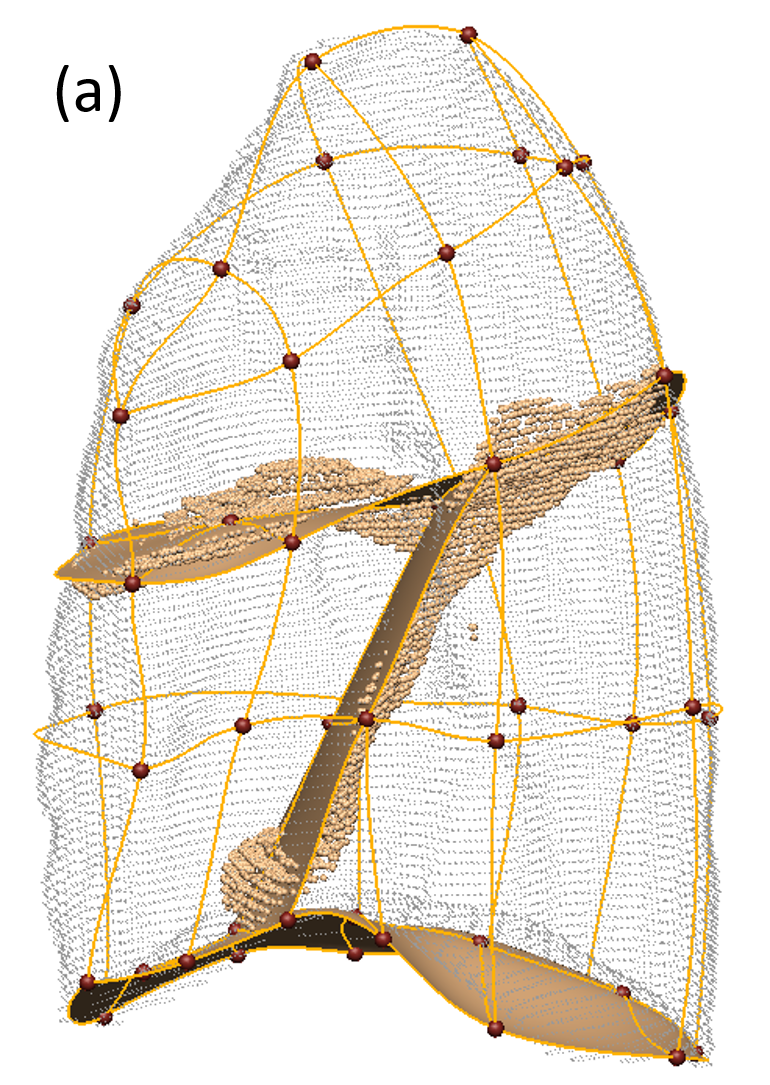
\includegraphics{Image/LobeFitting2.png}}
  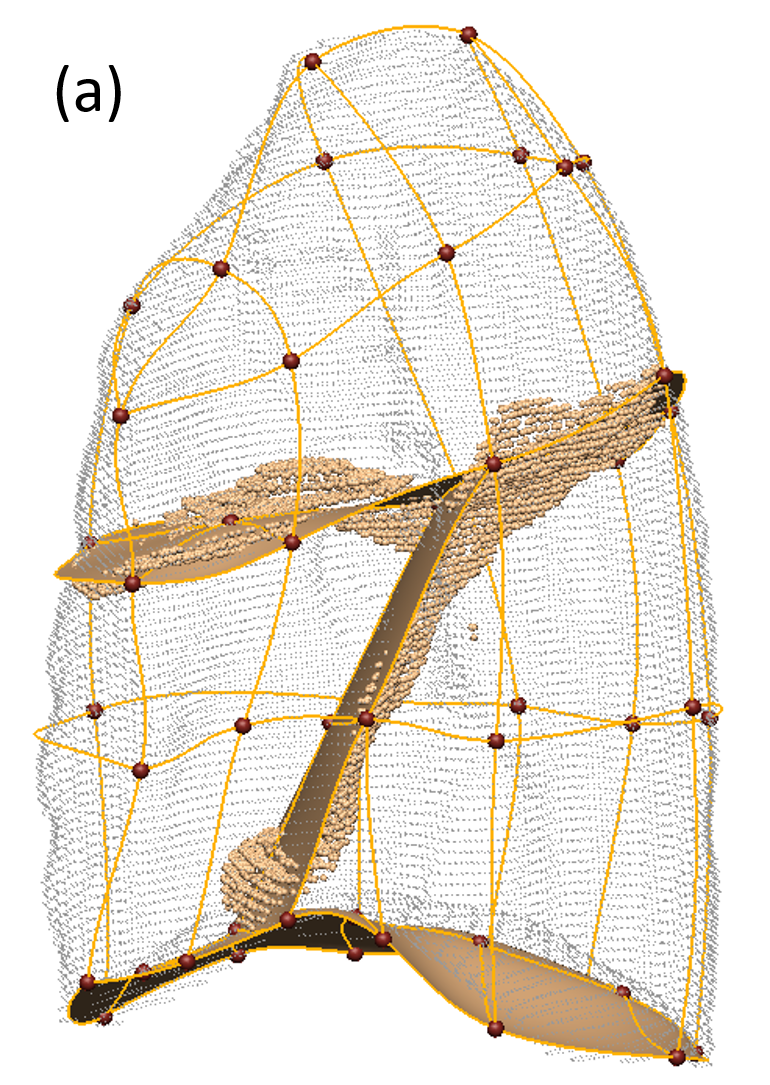
\includegraphics[width=\linewidth,trim={{.0\wd0} {.0\wd0} {.0\wd0} {.0\wd0}},clip]{Image/LobeFitting2.png}
  \centerline{}
  \label{fig:InitialFissurePrediction-a} 
	\end{minipage}
	}
\end{subfigure}
%\vspace{.3in} % control space between the upper context and figure
%\hspace{.2in} % control space between two figures
\begin{subfigure}{
  \begin{minipage}[t]{0.26\linewidth}
  \sbox0{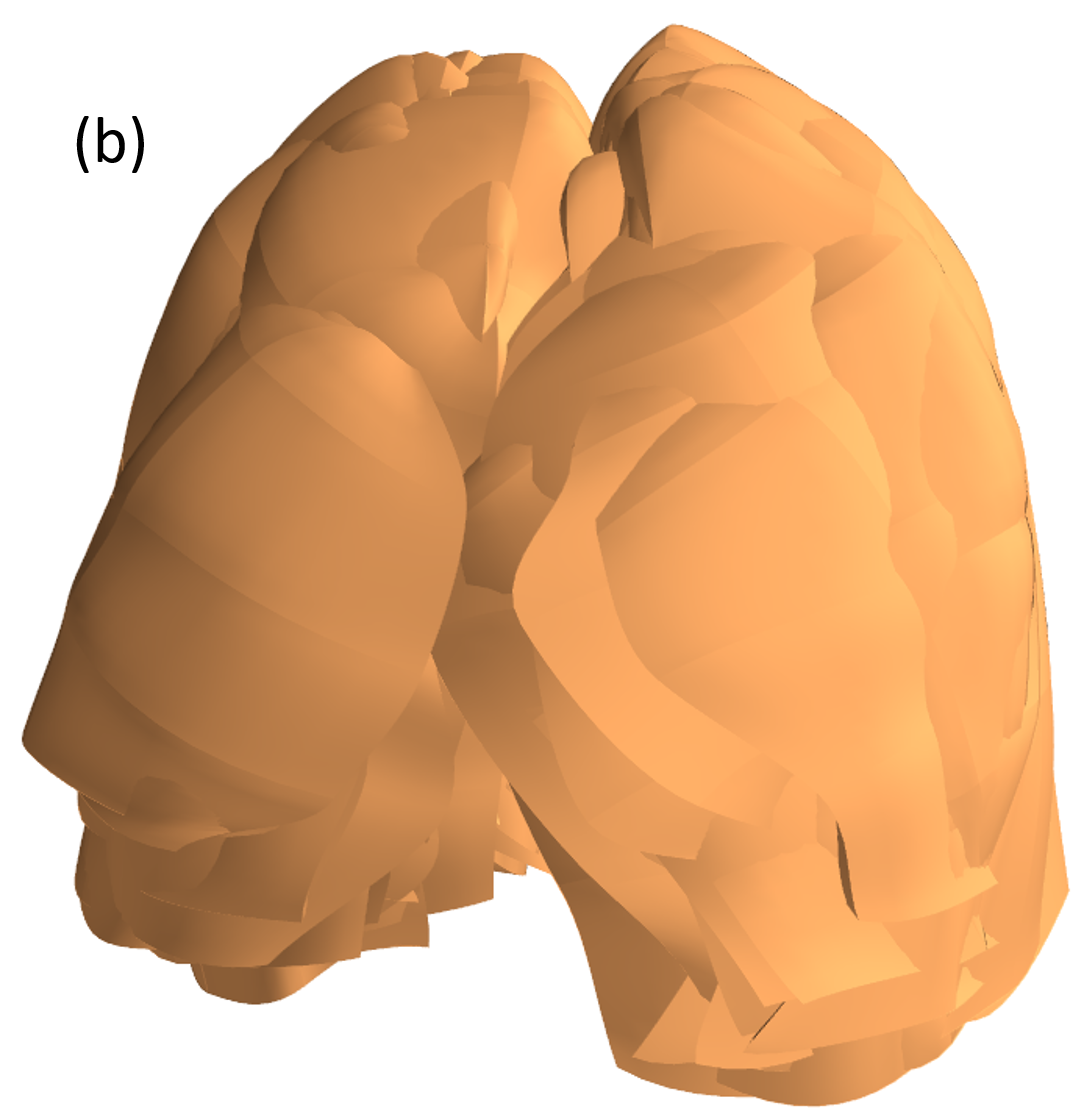
\includegraphics{Image/ProcrustedMeshes.png}}
  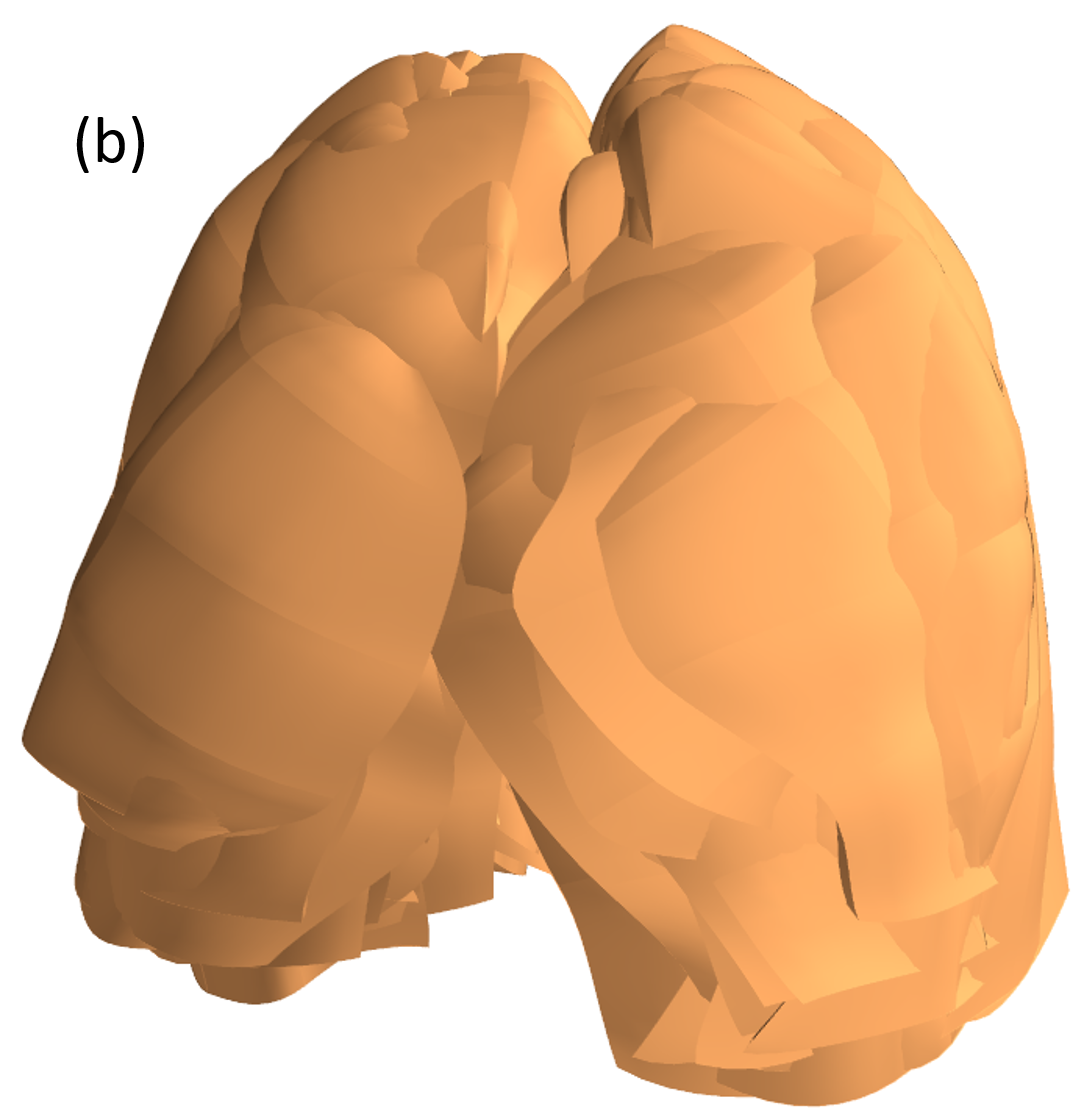
\includegraphics[width=\linewidth,trim={{.0\wd0} {.0\wd0} {.0\wd0} {.0\wd0}},clip]{Image/ProcrustedMeshes.png}
  \centerline{}
  \label{fig:InitialFissurePrediction-b} 
	\end{minipage}
	}
\end{subfigure}
\begin{subfigure}{
  \begin{minipage}[t]{0.18\linewidth}
  \sbox0{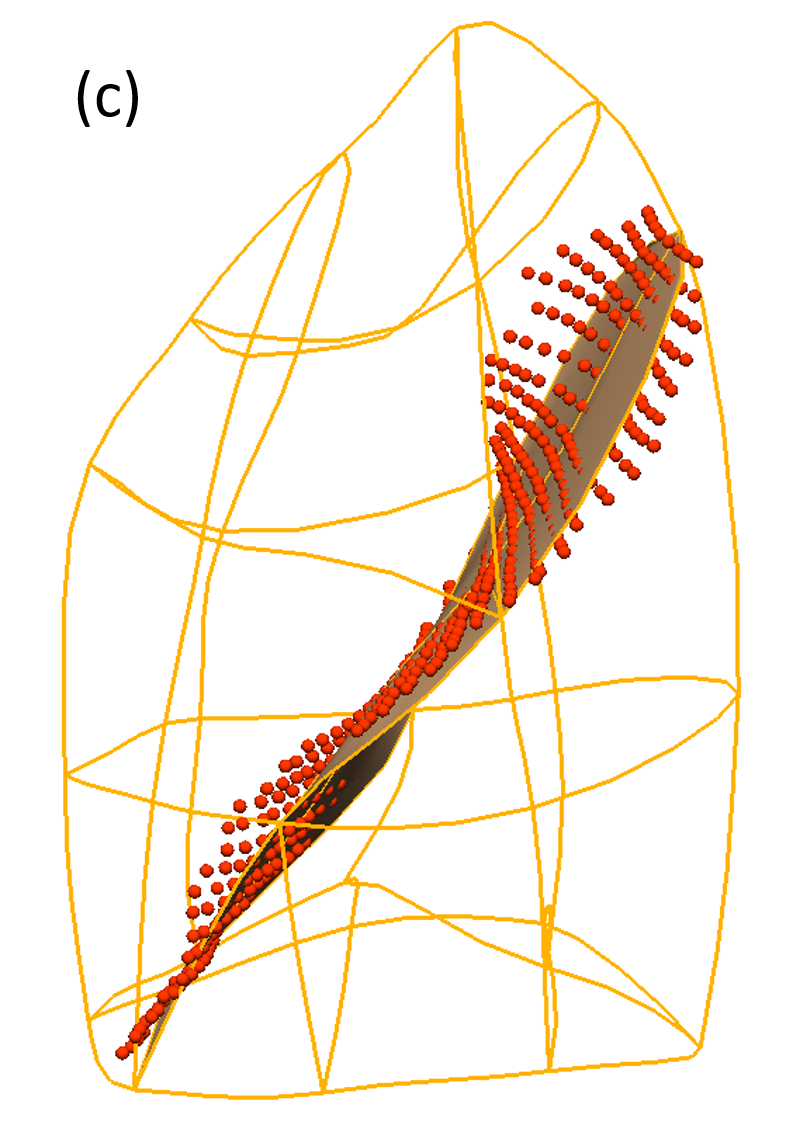
\includegraphics{Image/ProjectedLeftFissureMesh.png}}
  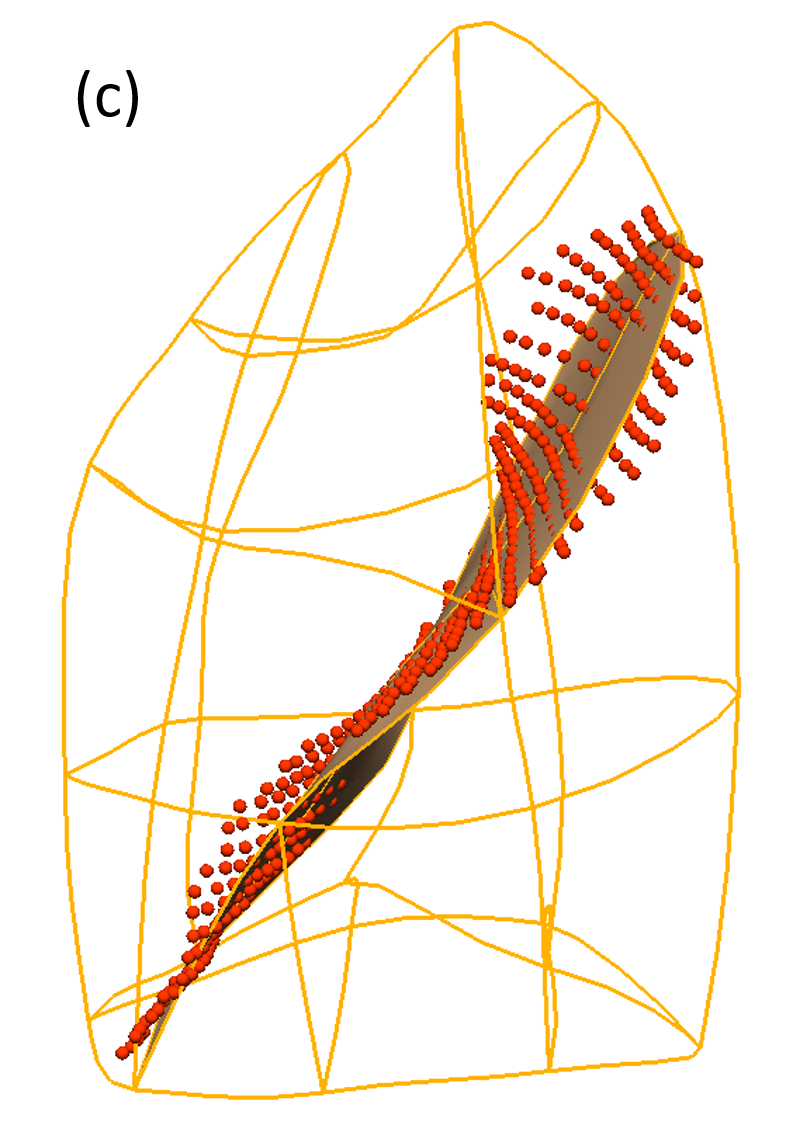
\includegraphics[width=\linewidth,trim={{.0\wd0} {.0\wd0} {.0\wd0} {.0\wd0}},clip]{Image/ProjectedLeftFissureMesh.png}
  \centerline{}
  \label{fig:InitialFissurePrediction-c}
	\end{minipage}
	}
\end{subfigure}
%\vspace{.3in} % control space between the upper context and figure
%\hspace{.2in} % control space between two figures
\begin{subfigure}{
  \begin{minipage}[t]{0.2\linewidth}
  \sbox0{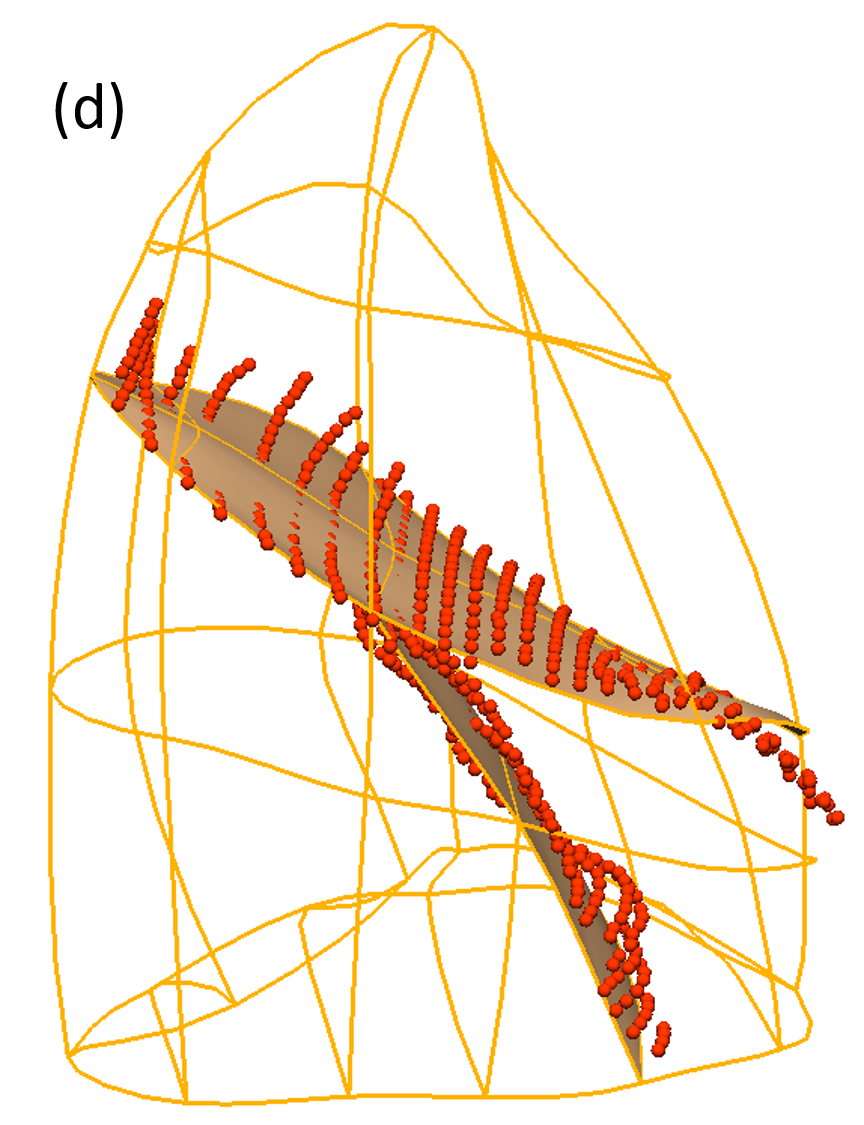
\includegraphics{Image/ProjectedRightFissureMesh.png}}
  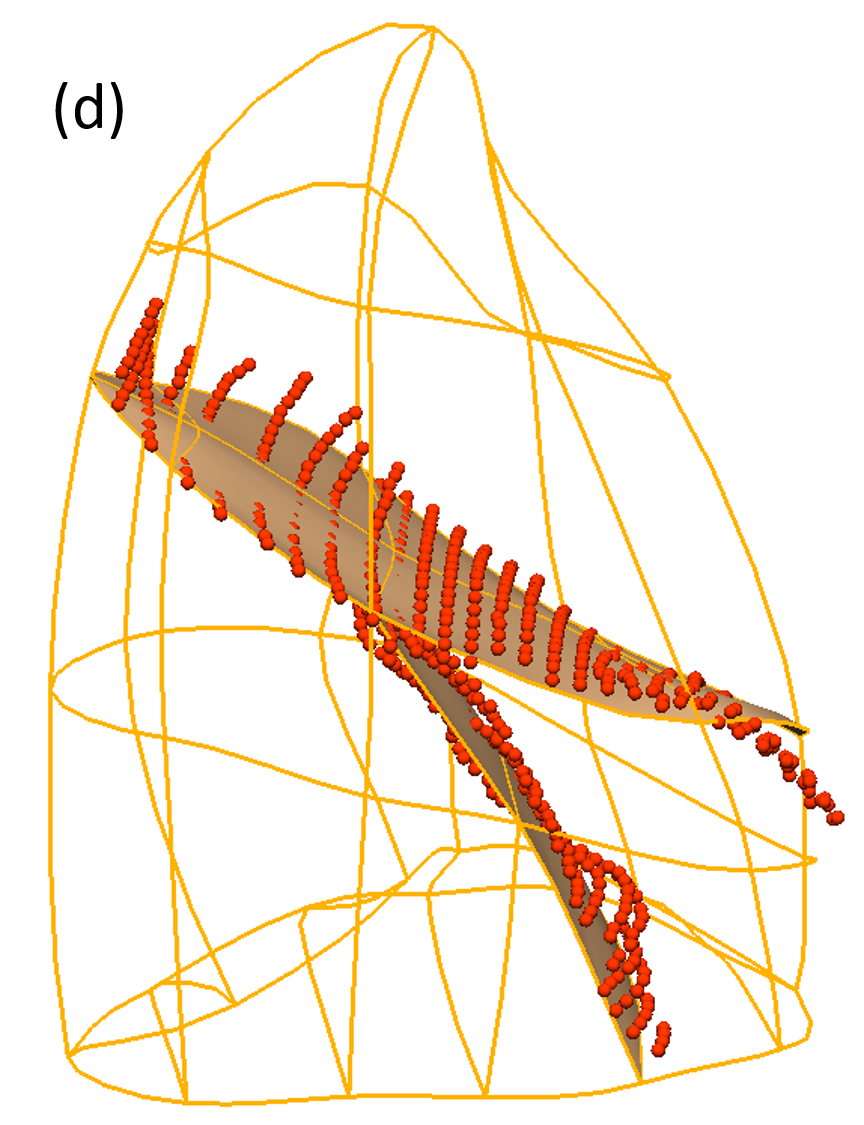
\includegraphics[width=\linewidth,trim={{.0\wd0} {.0\wd0} {.0\wd0} {.0\wd0}},clip]{Image/ProjectedRightFissureMesh.png}
  \centerline{}
  \label{fig:InitialFissurePrediction-d}
	\end{minipage}
	}
\end{subfigure}
\caption{SSM based initial fissure prediction. (a) Lung surface fitting and manually-digitized fissure data. (b) Procrustes aligned meshes of 50 subjects. (c) (d) Fissure predictions (gold surfaces) compared to ground truth fissure points.}
\label{fig:InitialFissurePrediction}
\end{figure}

\subsection{Multi-scale Hessian-based fissure detection}

This study used the Hessian matrix based on gray-scale curvature information combined with Gaussian smoothing as a basic operator to enhance the fissure structure. Gaussian filters with kernel sizes from 0.5-2.5 mm in 0.5 mm increments were applied to the image set. The responses at each kernel were combined to get a maximum response for each voxel of the image. This multi-scale operation guarantees fissures of variable size can be captured by Hessian operations. At each image voxel, the Hessian matrix was constructed from the six independent second order derivatives as a symmetric matrix. In 3D space, a fissure structure which presents as a light plane on a dark background, is characterized by one large positive second derivative ($\lambda_3$) perpendicular to the fissure plane, since the grey-value increases rapidly from the plane-structure border to the centreline and decreases again to the opposite border. And two small second derivatives of either sign ($\lambda_1$ and $\lambda_2$) parallel to the plane should occur. Thus, on the bright fissures, the ideal relationship is defined as $\mid\lambda_{1}\mid = \mid\lambda_{2}\mid = 0$ and $\lambda_{3} \ll 0$, $\mid\lambda_{1}\mid\leq\mid\lambda_{2}\mid\leq\mid\lambda_{3}\mid$ ($\lambda_3$ is expected to be much larger than $\lambda_1$ and $\lambda_2$). From these characteristics, the fissure probability of each voxel is

\begin{equation}
\label{eq:FissureHessian1}
F_0(s) = \Theta S_{plane} S_{noise}.
\end{equation}

The parameter $\Theta$ supresses points whose largest eigenvalue $\lambda_{3}$ is positive, since fissures are locally bright , and is defined as

\begin{equation}
\label{eq:FissureHessian2}
\Theta = \begin{cases}
         1,\quad \lambda_{3}< 0\\,
         0, \quad \lambda_{3}\geq0.
         \end{cases}
\end{equation}

Since the largest eigenvalue $\mid\lambda_{3}\mid$ should be much larger than the other two eigenvectors, the second factor $S_{plane}$ uses the ratio between $\mid\lambda_{2}\mid$ and $\mid\lambda_{3}\mid$ to search sheet-like structures, so that the voxels where $\mid\lambda_{3}\mid$ and $\mid\lambda_{2}\mid$ are significantly different. $S_{plane}$ is defined as

\begin{equation}
\label{eq:FissureHessian3}
S_{plane} = exp(-\frac{{R_{plane}}^2}{2\alpha^2}), \\
\end{equation}

\begin{equation}
\label{eq:FissureHessian4}
R_{plane} = \frac{\mid\lambda_{2}\mid}{\mid\lambda_{3}\mid},
\end{equation}

\noindent where $\alpha$ was set to 0.5 in this study. The third factor $S_{noise}$ aims to suppress noise voxels such as blob-like structures. Unlike plane-like structures which have relatively large $\mid\lambda_{2}\mid$ and $\mid\lambda_{3}\mid$ ratio, the noise voxels usually have low $\mid\lambda_{1}\mid$, $\mid\lambda_{2}\mid$ and $\mid\lambda_{3}\mid$. Therefore, here we use

\begin{equation}
\label{eq:FissureHessian5}
S_{noise} = 1 - exp(-\frac{{R_{noise}}^2}{2\beta^2}), \\
\end{equation}

\begin{equation}
\label{eq:FissureHessian6}
R_{noise} = \sqrt{{\lambda_1}^2+{\lambda_2}^2+{\lambda_3}^2},
\end{equation}

\noindent with $\beta$ set to 0.5 for thresholding. $F_0(s)$ then gives a high response to local plane-like structures (fissures) and suppresses other pulmonary structures (noise). An example of this enhancement filter applied in an individual is shown in Figure \ref{fig:FissureDetection-a}. Blood vessels are removed from the fissure enhanced result using a multiple scale (from 0.5 mm to 3.0 mm in 0.5 mm increments as the kernel size of Gaussian) Hessian-based enhanced filter. In a 3D image, blood vessels, appear as ideal bright tubular structures in a dark background, should be described as $\mid\lambda_{1}\mid\approx$ 0, $\mid\lambda_{1}\mid\ll\mid\lambda_{2}\mid$,  $\lambda_{2}\approx\lambda_{3}$ \cite{frangi1998multiscale}. Figure \ref{fig:FissureDetection-b} shows the result after eliminating the vessel voxels.

The initial fissure location predicted by average SSM deformation gives a region of interest (ROI) for an accurate fissure detection, see Figure \ref{fig:FissureDetection-c}. The candidate points are selected within a certain distance of the initial fissure approximation: the search distance was set to 20 voxels (default value) for the initially projected left and right oblique fissures and 15 voxels for the initially projected right horizontal fissure. To remove some spurious responses such as small plane-like structures on the result, a 2D 4-neighbourhood connected component filter and a 3D 6-neighbourhood vector-based connected component filter were employed successively to eliminate noise arising from small plane-like structures in this search region (Fig \ref{fig:FissureDetection-d}). A 2D filter was used to eliminate 4-neighbour connected components that were smaller than a minimum small size (set to 10 voxels initially) slice by slice. The 3D vector-based connected component filter uses the inner product of the normalized largest eigenvector of the Hessian matrix in adjacent voxels. These largest eigenvectors are perpendicular to the fissure plane, and their inner product provides a criterion for component connection. As the curvature of a fissure is locally low, adjacent fissure voxels should have similar largest eigenvectors and thus the inner product value of their largest eigenvectors should equal to 1 or slightly smaller than 1. Connected boundary condition was set as an inner product $\leq$ 0.8 to connected component, then 3D 6-neighbour connected component with a volume less than 100 $\mathrm{mm^3}$ was removed as noise from the result.

The detected points were then divided into a set of small subsections corresponding to different x, y intervals. For each subsection, the point of the highest fissure probability (the highest S value) was selected as the final candidate fissure point (Fig \ref{fig:FissureDetection-e}). Once the maximum fissureness candidates were found, a morphological dilation with a $3\times3\times3$ voxel cube as structure element was applied iteratively until the largest connected fissure plane was big enough, so that all the other unconnected outliers could be filtered subsequently. Finally, a continuous smooth fissure surface was generated based on the maximum fissure points using a $\beta$-spline method with a thin-plane spline \cite{lee1997scattered} and extrapolated to the lung boundaries, see Fig \ref{fig:FissureDetection-f}.

\begin{figure}[htbp] 
\centering
\begin{subfigure}{
  \begin{minipage}[t]{0.295\linewidth}
  \sbox0{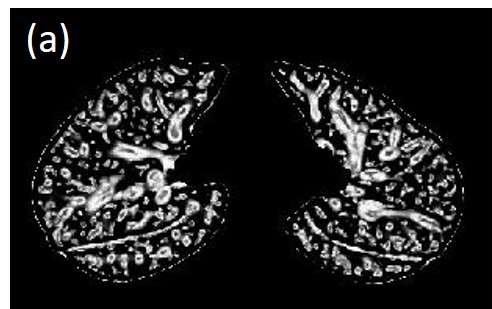
\includegraphics{Image/FissureDetection1.jpg}} 
  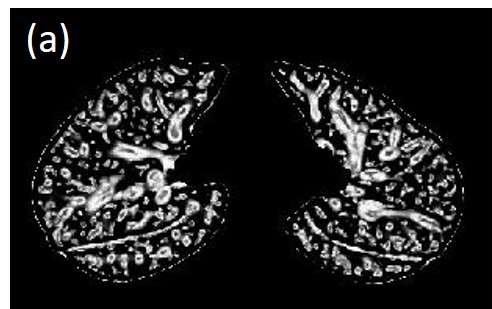
\includegraphics[width=\linewidth,trim={{.0\wd0} {.0\wd0} {.0\wd0} {.0\wd0}},clip]{Image/FissureDetection1.jpg} %trim={<left> <lower> <right> <upper>}, set the cut scale
  \centerline{}
	\label{fig:FissureDetection-a}
	\end{minipage}%
   }%
\end{subfigure} 
\begin{subfigure}{
  \begin{minipage}[t]{0.288\linewidth}
  \sbox0{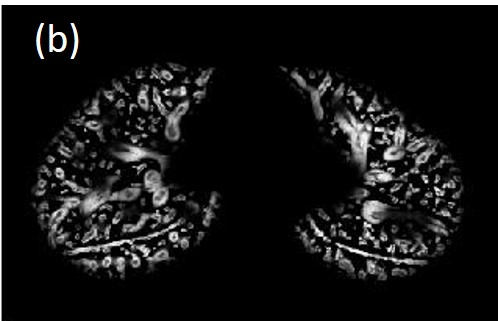
\includegraphics{Image/FissureDetection2.jpg}}
  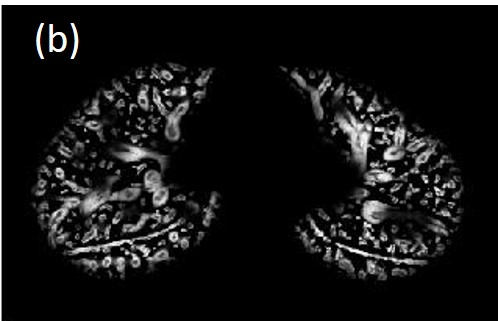
\includegraphics[width=\linewidth,trim={{.0\wd0} {.0\wd0} {.0\wd0} {.0\wd0}},clip]{Image/FissureDetection2.jpg}
  \centerline{}
	\label{fig:FissureDetection-b}
	\end{minipage}%
   }%
\end{subfigure}
\begin{subfigure}{
  \begin{minipage}[t]{0.288\linewidth}
  \sbox0{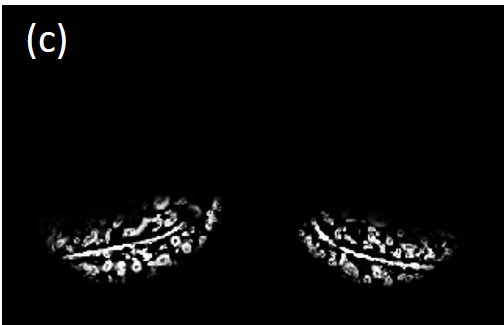
\includegraphics{Image/FissureDetection3.jpg}}
  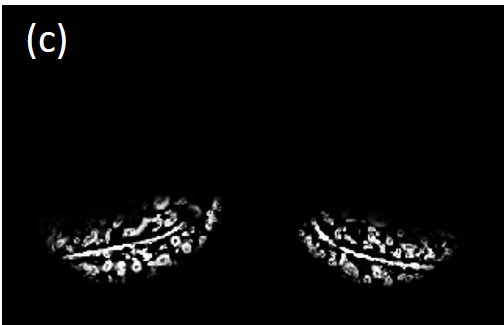
\includegraphics[width=\linewidth,trim={{.0\wd0} {.0\wd0} {.0\wd0} {.0\wd0}},clip]{Image/FissureDetection3.jpg}
  \centerline{}
	\label{fig:FissureDetection-c}
	\end{minipage}%
   }%
\end{subfigure}
\begin{subfigure}{
  \begin{minipage}[t]{0.287\linewidth}
  \sbox0{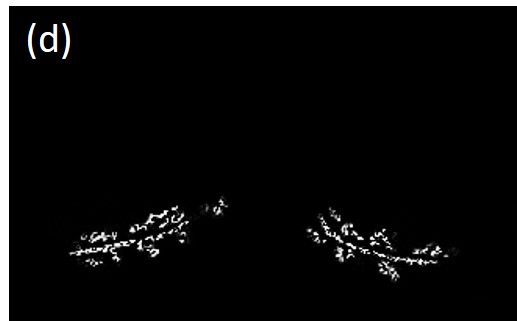
\includegraphics{Image/FissureDetection4.jpg}}
  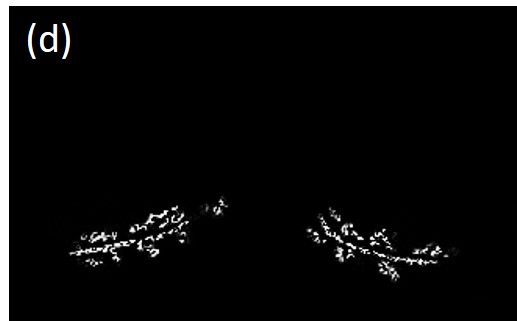
\includegraphics[width=\linewidth,trim={{.0\wd0} {.0\wd0} {.0\wd0} {.0\wd0}},clip]{Image/FissureDetection4.jpg}\label{fig:FissureDetection}
  \centerline{}
	\label{fig:FissureDetection-d}
	\end{minipage}%
   }%
\end{subfigure}
\begin{subfigure}{
  \begin{minipage}[t]{0.30\linewidth}
  \sbox0{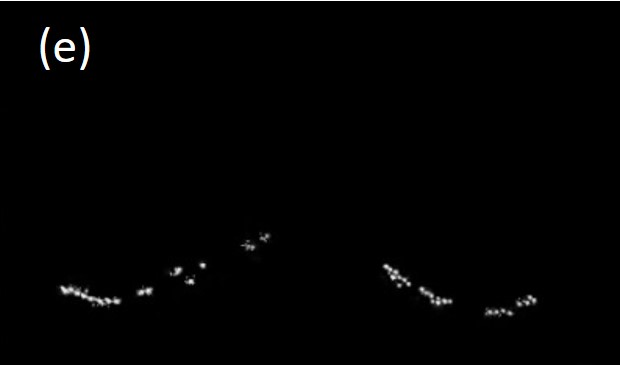
\includegraphics{Image/FissureDetection5.jpg}}
  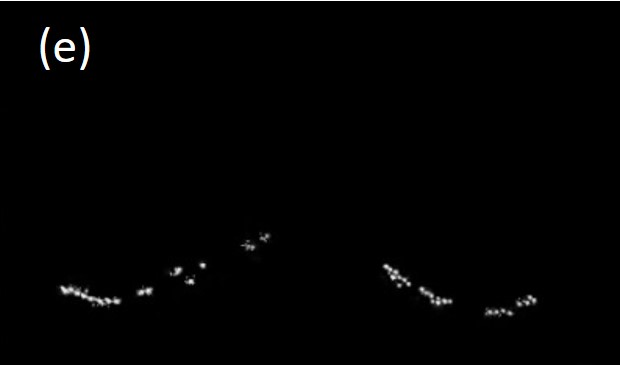
\includegraphics[width=\linewidth,trim={{.0\wd0} {.0\wd0} {.0\wd0} {.0\wd0}},clip]{Image/FissureDetection5.jpg}
  \centerline{}
	\label{fig:FissureDetection-e}
	\end{minipage}%
   }%
\end{subfigure}
\begin{subfigure}{
  \begin{minipage}[t]{0.305\linewidth}
  \sbox0{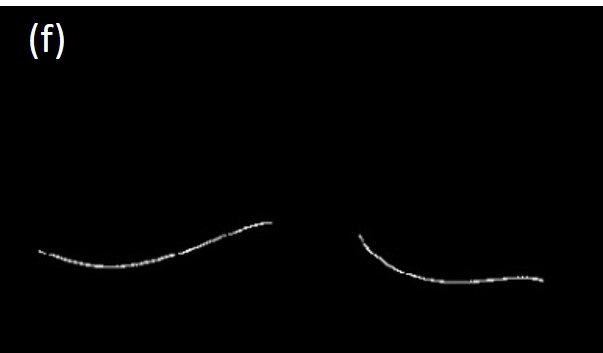
\includegraphics{Image/FissureDetection6.jpg}}
  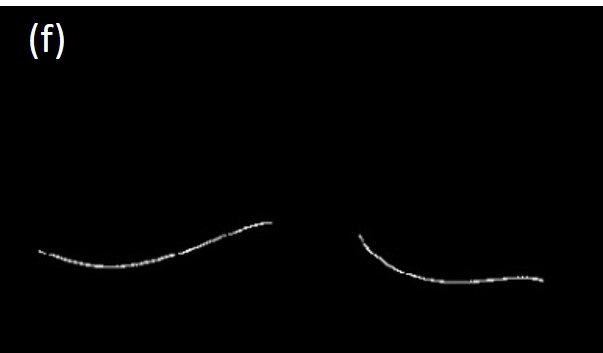
\includegraphics[width=\linewidth,trim={{.0\wd0} {.0\wd0} {.0\wd0} {.0\wd0}},clip]{Image/FissureDetection6.jpg}
  \centerline{}
	\label{fig:FissureDetection-f}
	\end{minipage}%
   }%
\end{subfigure}
\caption{Hessian-based multiscale fissure detection results. (a) Hessian-based plane-like structure enhancement filter. (b) Remove vessel voxels (tube-like structures). (c) Selected search regions for fissure detection based on SSM initial fissure prediction. (d) 2D and 3D eigenvector based connected component filter. (e) Fissure candidate points. (f) $\beta$-spline curve fissure surface fitting.}
\label{fig:FissureDetection}
\end{figure}

\section{RESULTS}
\label{SegmentationExperiment}
 
\subsection{Testing CT dataset}

The semi-automatic SSM lobe segmentation method was tested on two datasets: 1) CT images from five young normal subjects taken at different lung volumes (end inspiration and end expiration), in the supine posture, from the HLA dataset (introduced in Section \ref{ShapeModelGeneration}). The selected dataset consists of five end expiration images and five end inspiration images, which were not part of the SSM training set; 2) CT images from older patients (slice thickness 1.25-3.00 mm) acquired during routine diagnostic inspection for idiopathic pulmonary fibrosis (IPF). Data from these subjects were acquired from the Auckland District Health Board (ADHB. Access to clinical data was approved by the Southern Health and Disability Ethics Committee. 

\subsection{Test and results}
Figure \ref{fig:HLASegmentationResults} shows raw images, initial SSM based fissure predicted locations, and the final automatic SSM-based lobar segmentation results for a normal healthy subject.  

\begin{figure}[htbp] 
\centering
\begin{subfigure}{
  \begin{minipage}[t]{0.15\linewidth}
  \sbox0{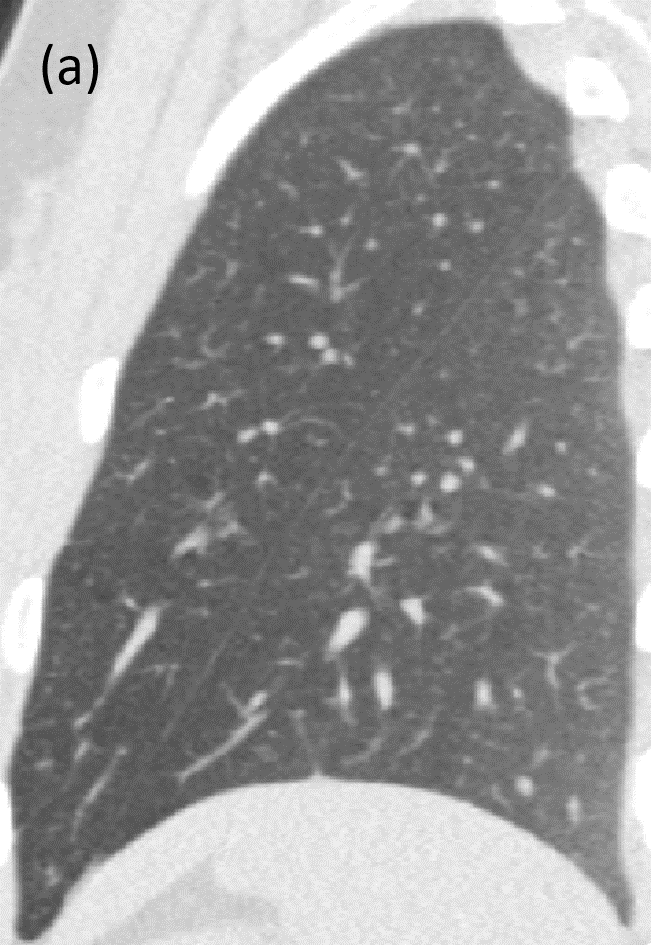
\includegraphics{Image/H1335_FRC_Raw_Sagittal.png}}
  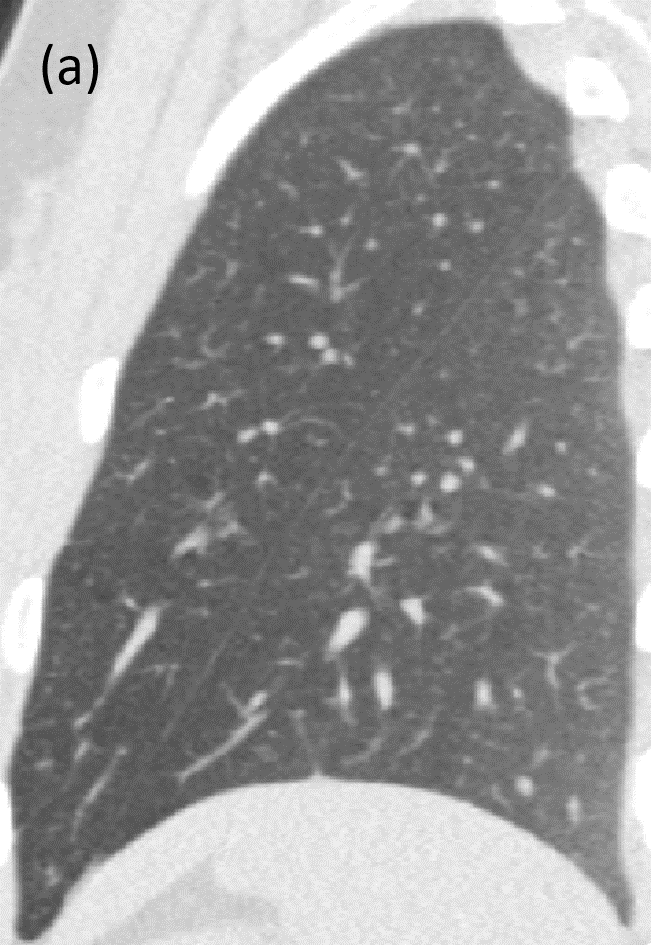
\includegraphics[width=\linewidth,trim={{.0\wd0} {.0\wd0} {.0\wd0} {.0\wd0}},clip]{Image/H1335_FRC_Raw_Sagittal.png}
  \centerline{}
	\end{minipage}%
   }%
  \label{fig:HLASegmentationResults-a} 
\end{subfigure}
%\vspace{.1in} % control space between the upper context and figure
%\hspace{.3in} % control space between two figures
\begin{subfigure}{
  \begin{minipage}[t]{0.15\linewidth}
  \sbox0{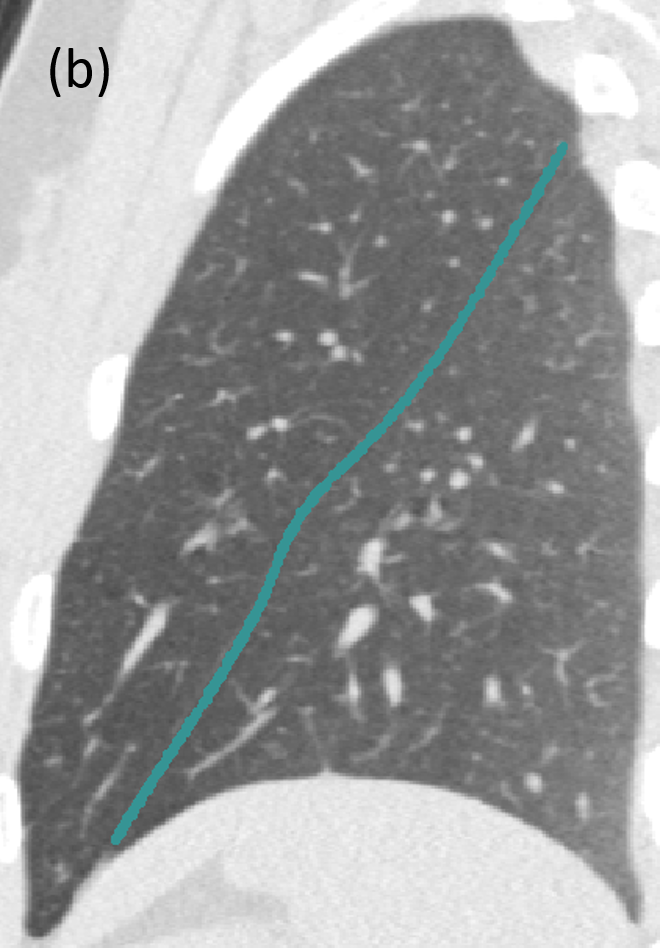
\includegraphics{Image/H1335_FRC_PCAInitial_Sagittal.png}}
  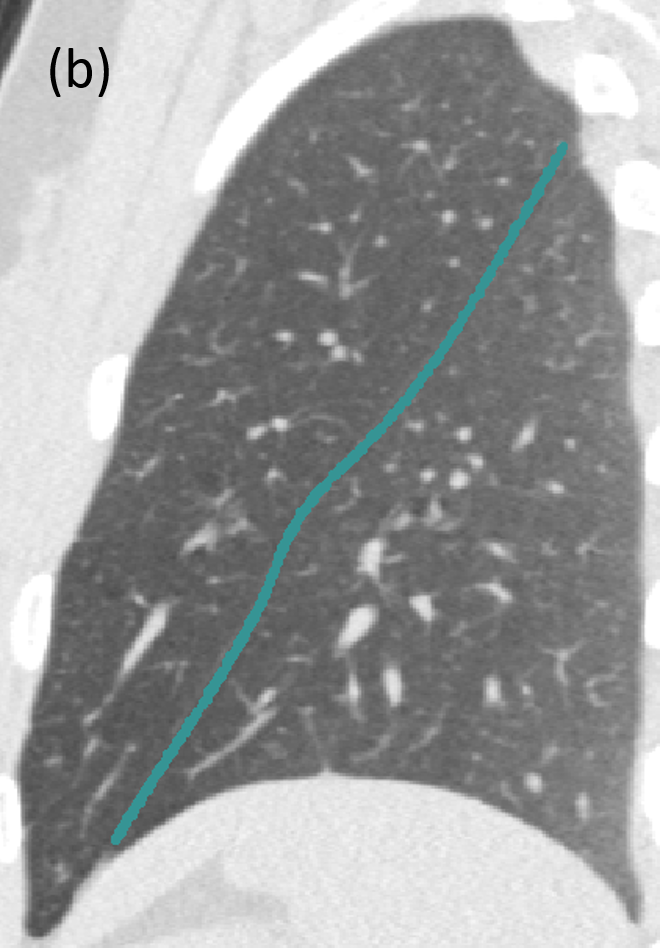
\includegraphics[width=\linewidth,trim={{.0\wd0} {.0\wd0} {.0\wd0} {.0\wd0}},clip]{Image/H1335_FRC_PCAInitial_Sagittal.png}
  \centerline{}
	\end{minipage}%
   }%
  \label{fig:HLASegmentationResults-b} 
\end{subfigure}
%\vspace{.1in} % control space between the upper context and figure
%\hspace{.3in} % control space between two figures
\begin{subfigure}{
  \begin{minipage}[t]{0.15\linewidth}
  \sbox0{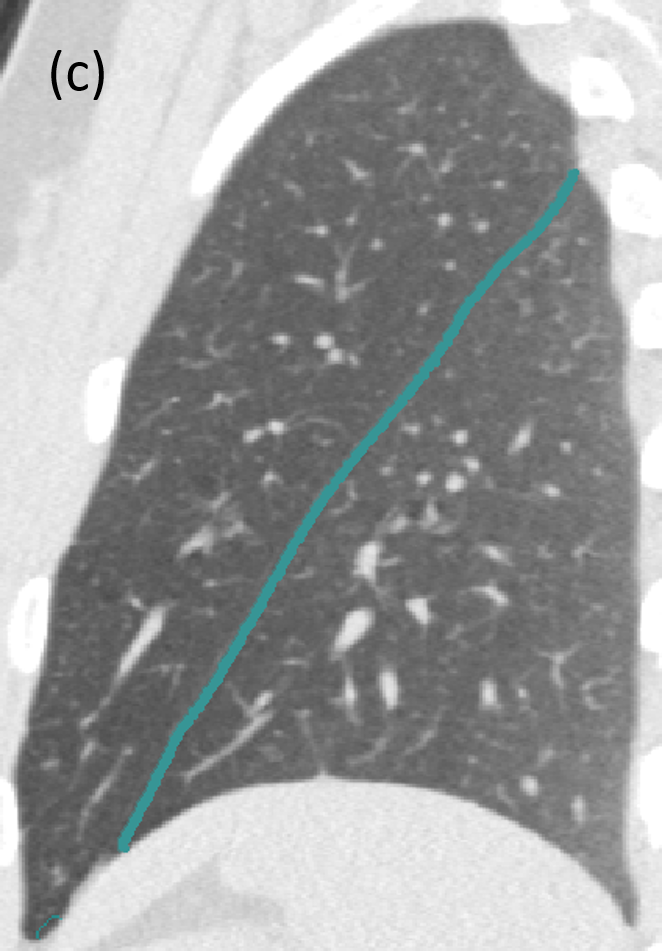
\includegraphics{Image/H1335_FRC_PCAFissureDetection_Sagittal.png}}
  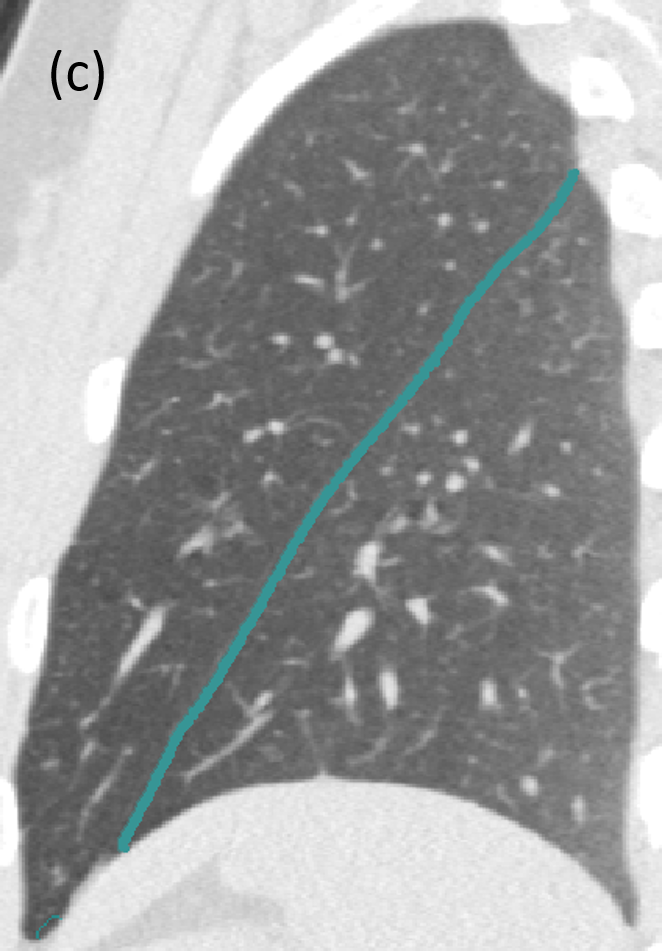
\includegraphics[width=\linewidth,trim={{.0\wd0} {.0\wd0} {.0\wd0} {.0\wd0}},clip]{Image/H1335_FRC_PCAFissureDetection_Sagittal.png}
  \centerline{}
	\end{minipage}%
   }%
  \label{fig:HLASegmentationResults-c} 
\end{subfigure}
\hspace{2.8in}
\vspace{.1in}
\begin{subfigure}{
 \begin{minipage}[t]{0.2\linewidth}
  \sbox0{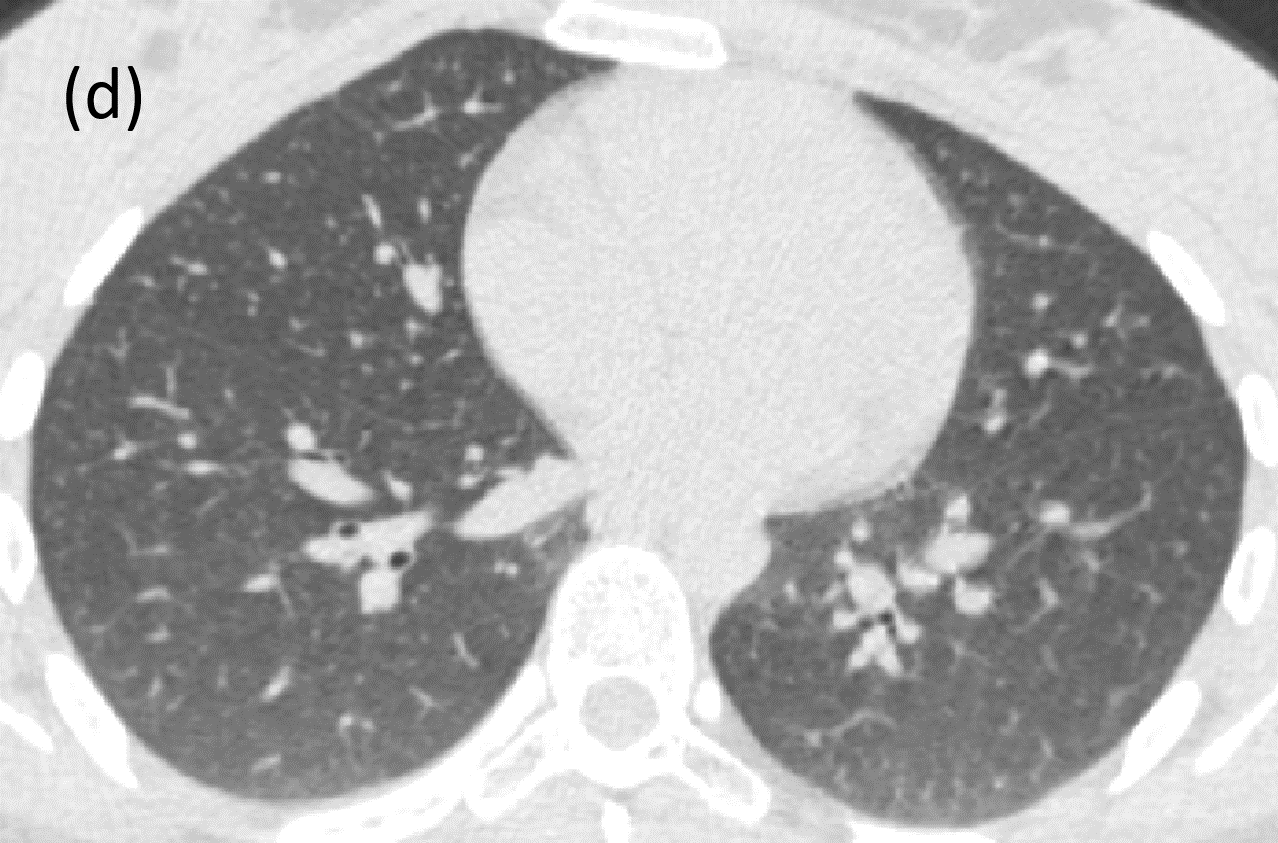
\includegraphics{Image/H1335_FRC_Raw_Axial.png}}
  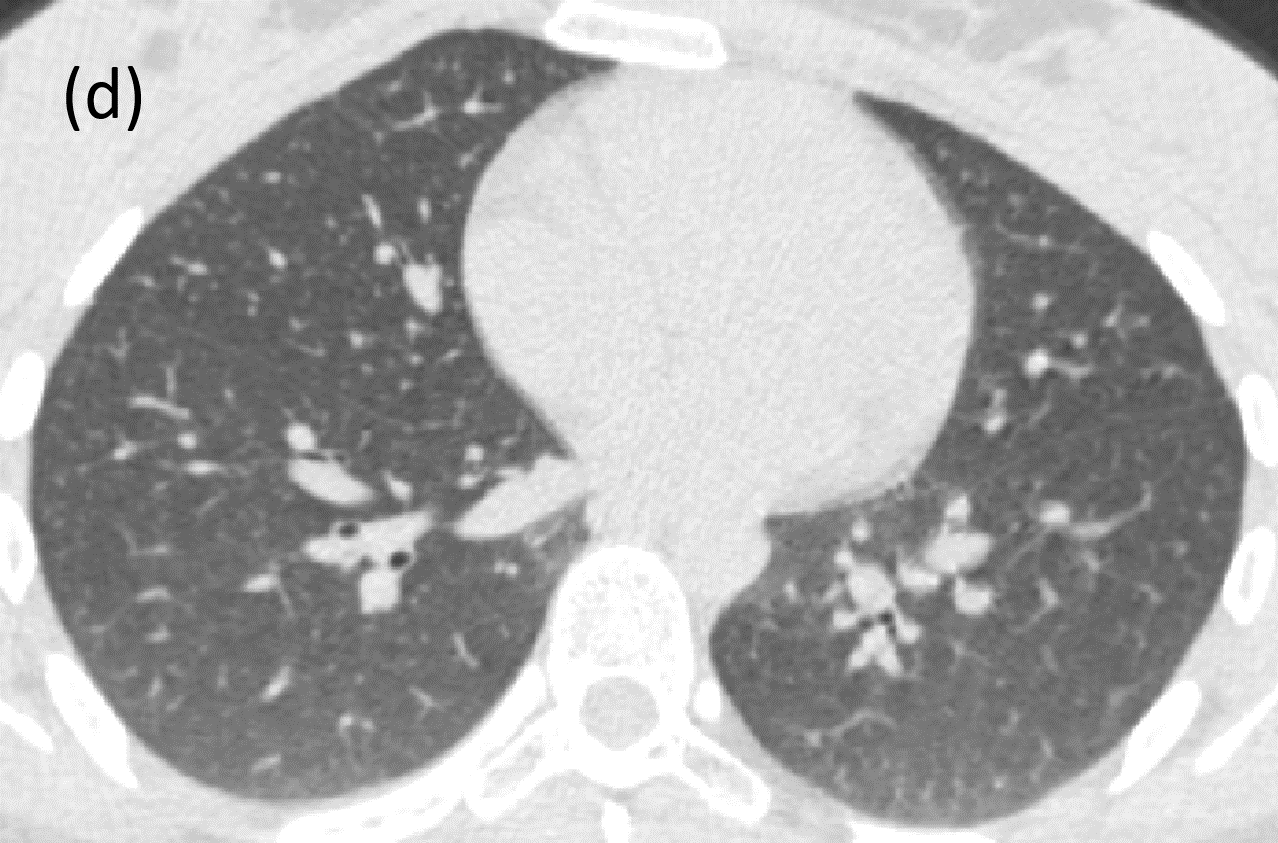
\includegraphics[width=\linewidth,trim={{.0\wd0} {.0\wd0} {.0\wd0} {.0\wd0}},clip]{Image/H1335_FRC_Raw_Axial.png}
  \centerline{}
	\end{minipage}%
   }%
  \label{fig:HLASegmentationResults-d} 
\end{subfigure}
%\vspace{.1in} % control space between the upper context and figure
%\hspace{.3in} % control space between two figures
\begin{subfigure}{
  \begin{minipage}[t]{0.2\linewidth}
  \sbox0{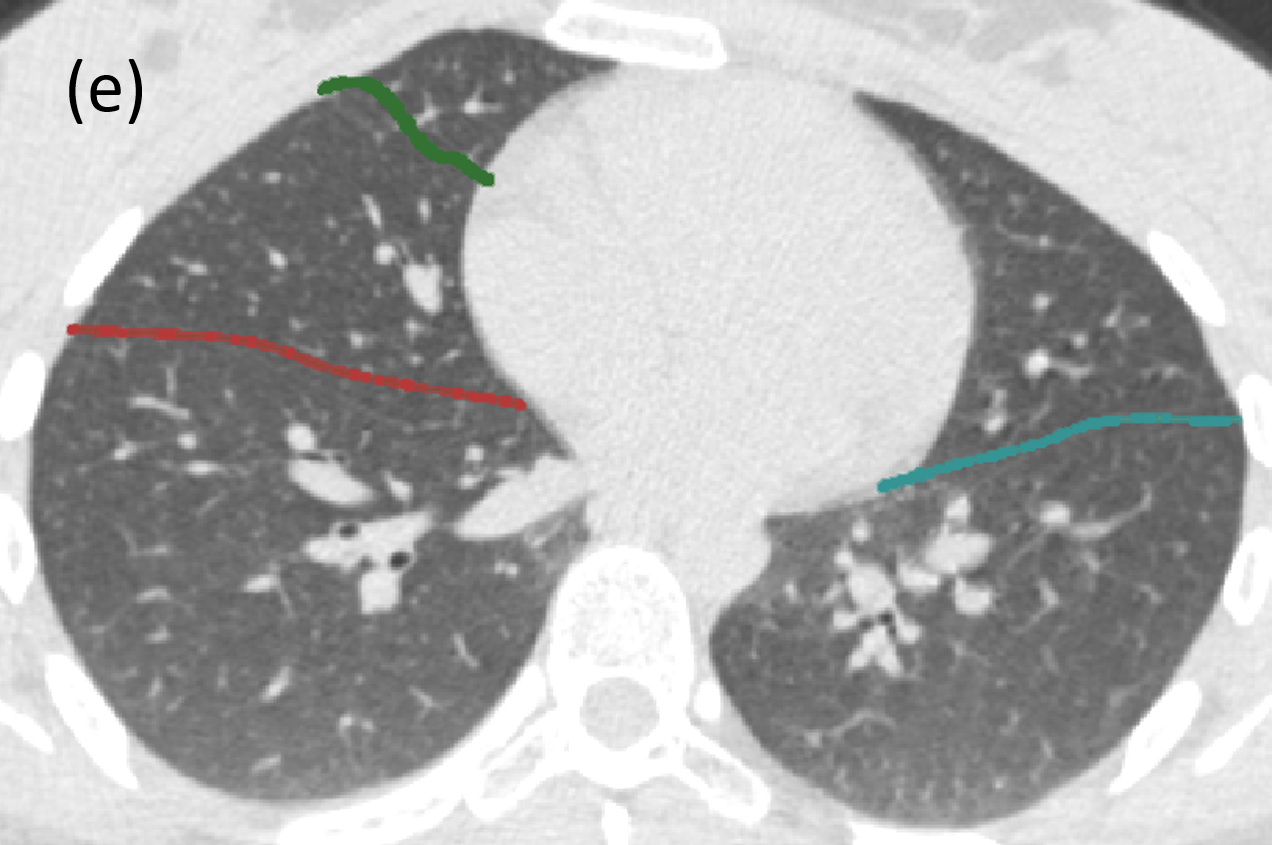
\includegraphics{Image/H1335_FRC_PCAInitial_Axial.png}}
  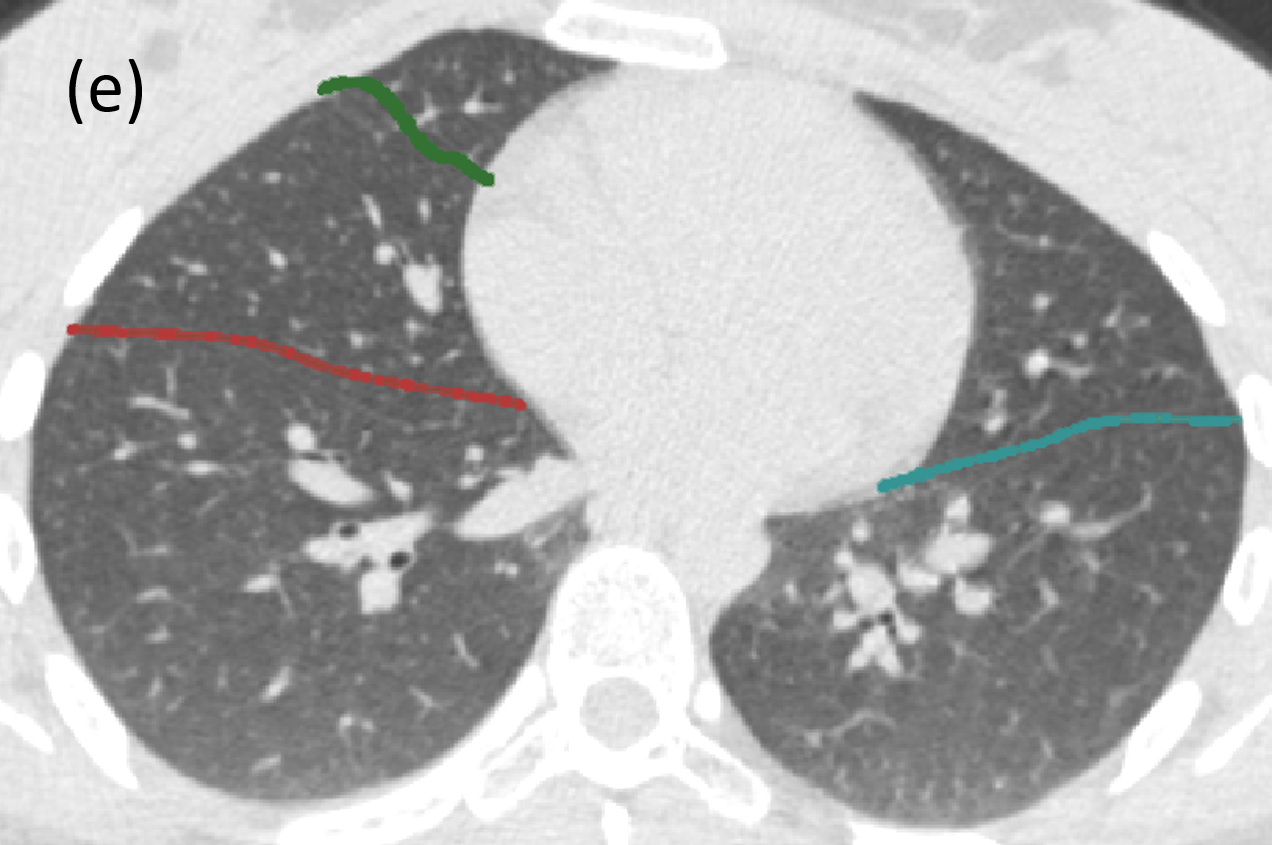
\includegraphics[width=\linewidth,trim={{.0\wd0} {.0\wd0} {.0\wd0} {.0\wd0}},clip]{Image/H1335_FRC_PCAInitial_Axial.png}
  \centerline{}
	\end{minipage}%
   }%
  \label{fig:HLASegmentationResults-e} 
\end{subfigure}
%\vspace{.1in} % control space between the upper context and figure
%\hspace{.3in} % control space between two figures
\begin{subfigure}{
  \begin{minipage}[t]{0.2\linewidth}
  \sbox0{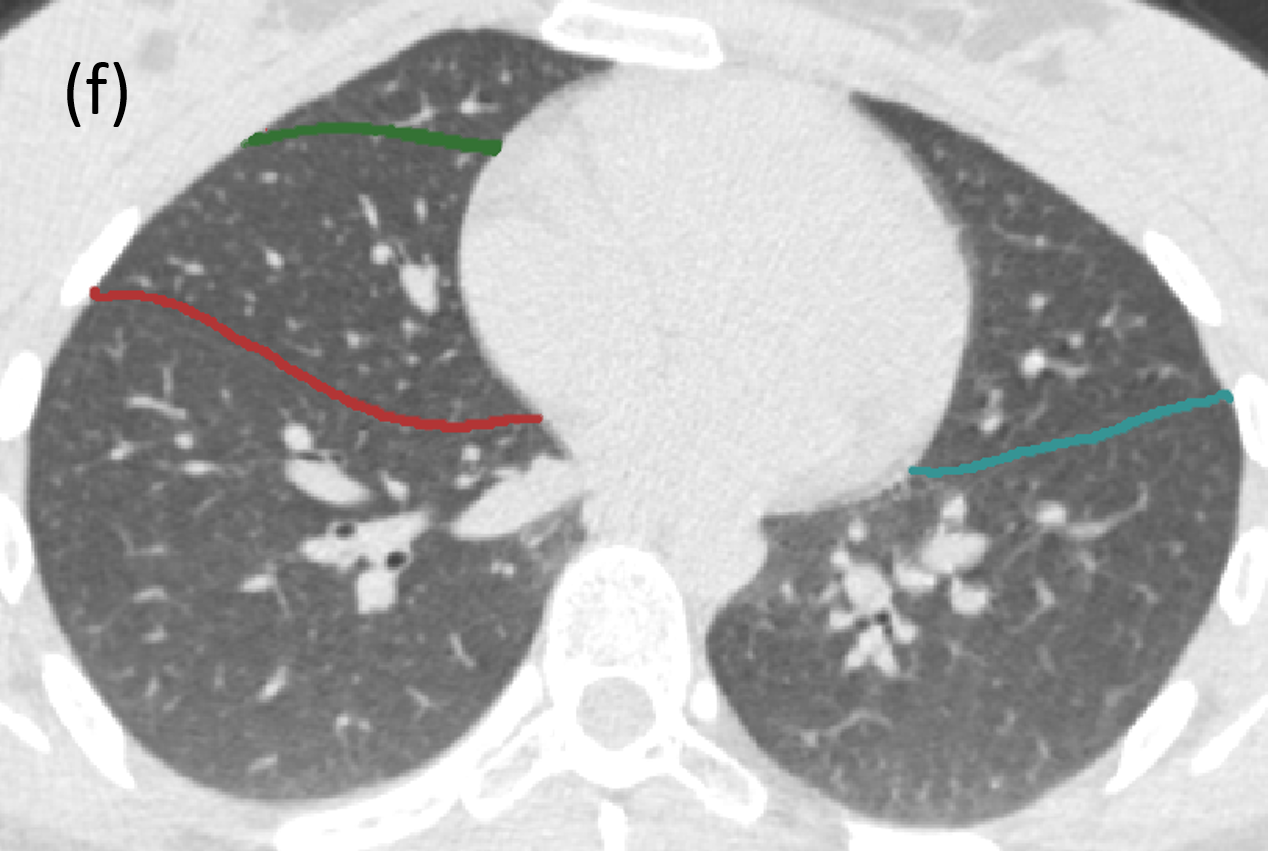
\includegraphics{Image/H1335_FRC_PCAFissureDetection_Axial.png}}
  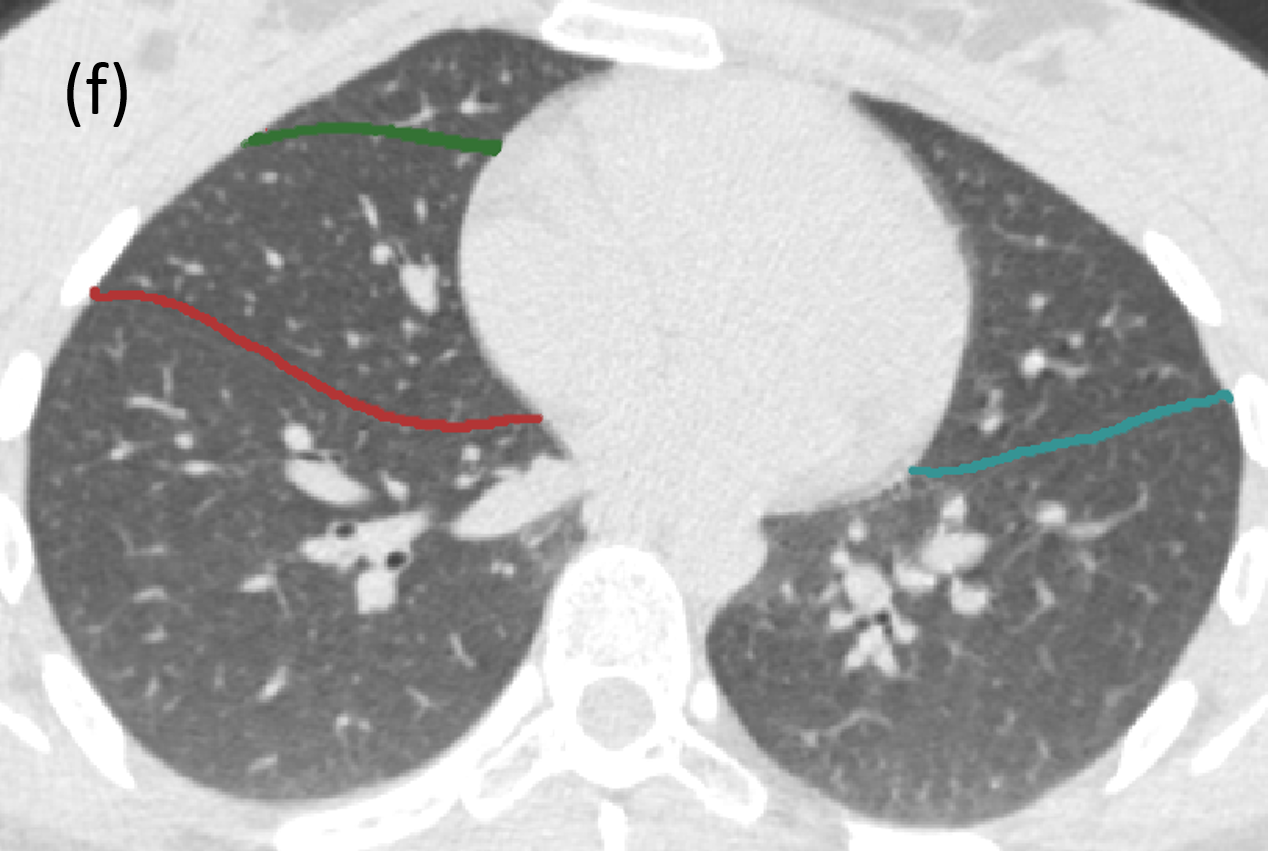
\includegraphics[width=\linewidth,trim={{.0\wd0} {.0\wd0} {.0\wd0} {.0\wd0}},clip]{Image/H1335_FRC_PCAFissureDetection_Axial.png}
  \centerline{}
	\end{minipage}%
   }%
  \label{fig:HLASegmentationResults-f} 
\end{subfigure}
\hspace{2.8in}
\vspace{.1in}
\begin{subfigure}{
  \begin{minipage}[t]{0.2\linewidth}
  \sbox0{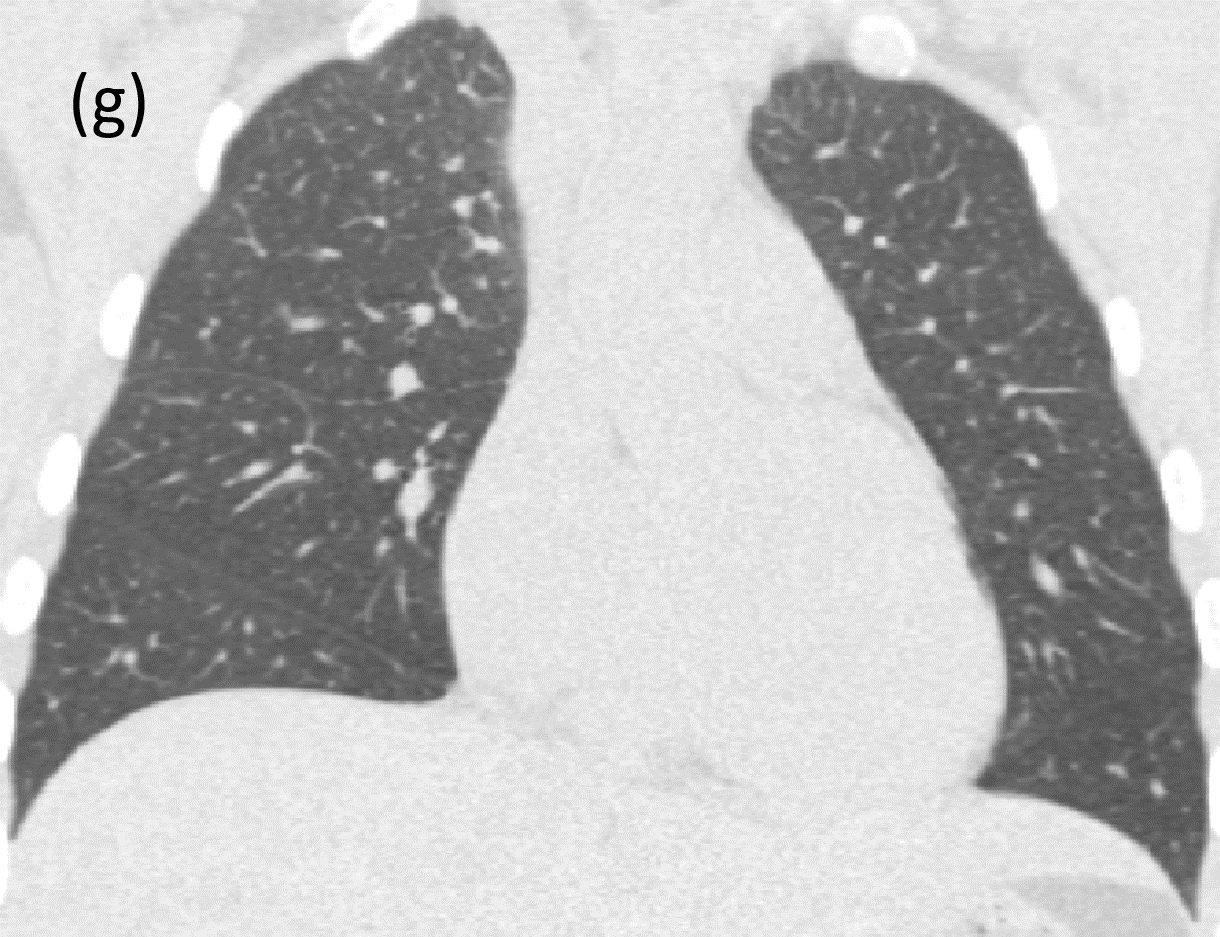
\includegraphics{Image/H1335_FRC_Raw_Coronal.png}}
  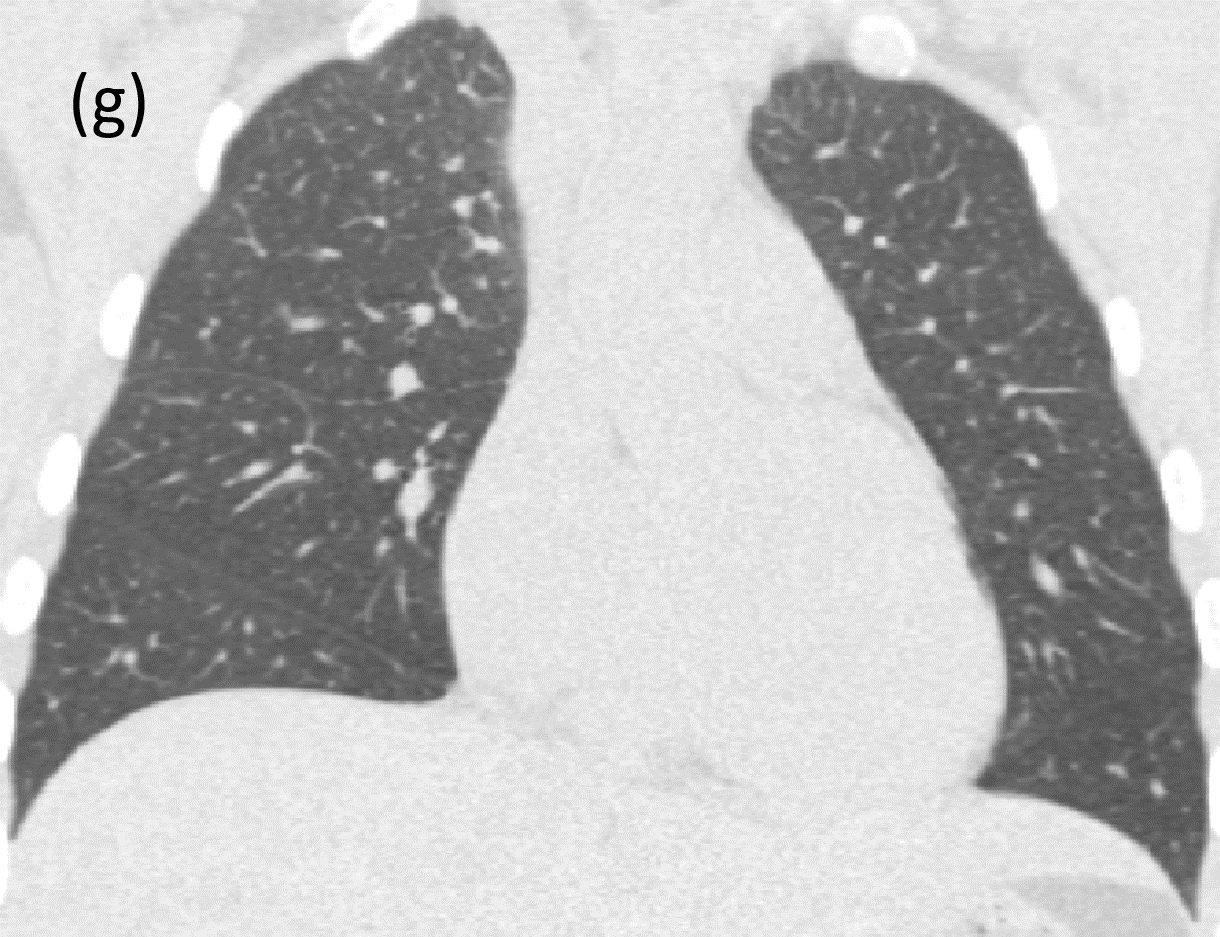
\includegraphics[width=\linewidth,trim={{.0\wd0} {.0\wd0} {.0\wd0} {.0\wd0}},clip]{Image/H1335_FRC_Raw_Coronal.png}
  \centerline{}
	\end{minipage}%
   }%
  \label{fig:HLASegmentationResults-g} 
\end{subfigure}
%\vspace{.1in} % control space between the upper context and figure
%\hspace{.3in} % control space between two figures
\begin{subfigure}{
  \begin{minipage}[t]{0.2\linewidth}
  \sbox0{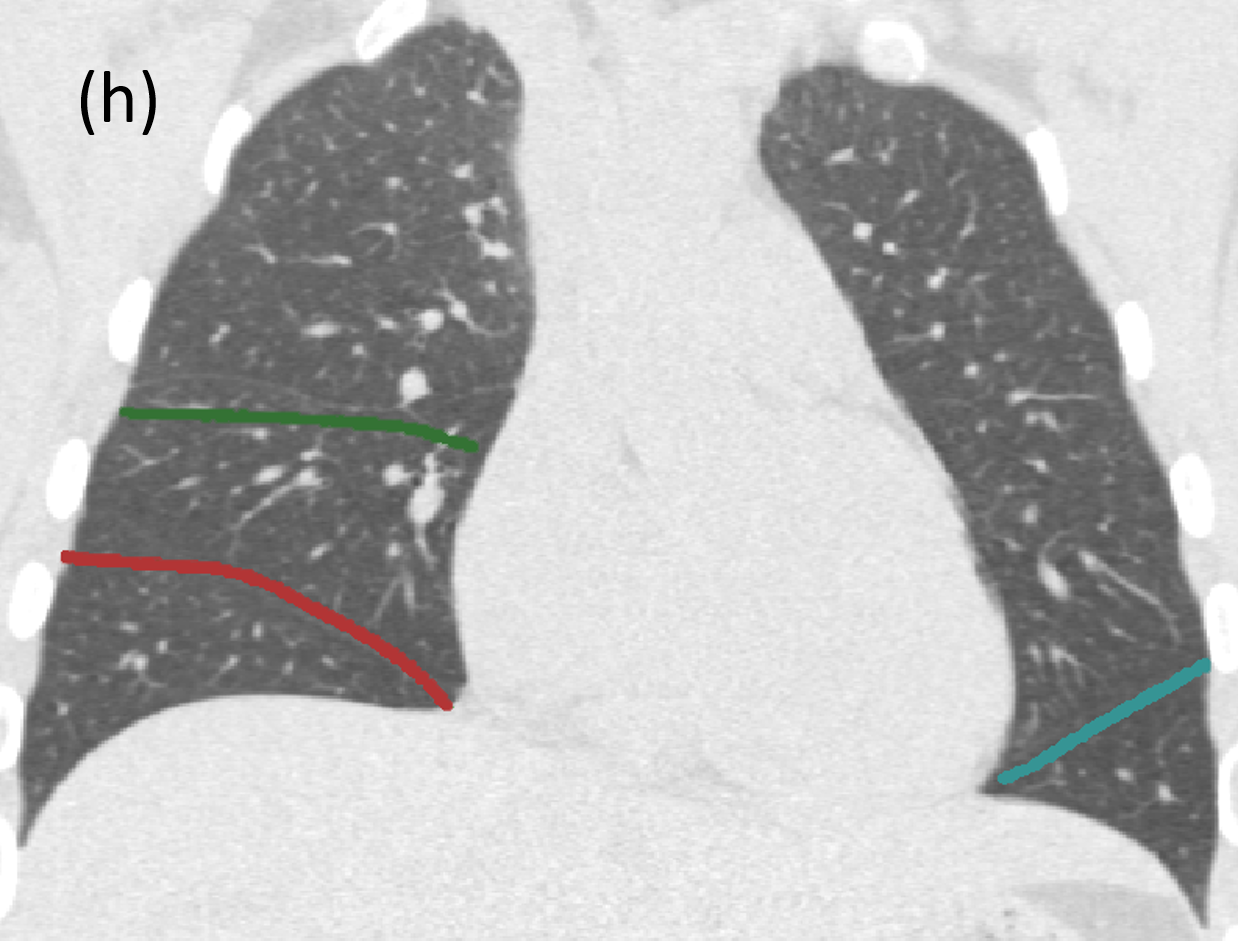
\includegraphics{Image/H1335_FRC_PCAInitial_Coronal.png}}
  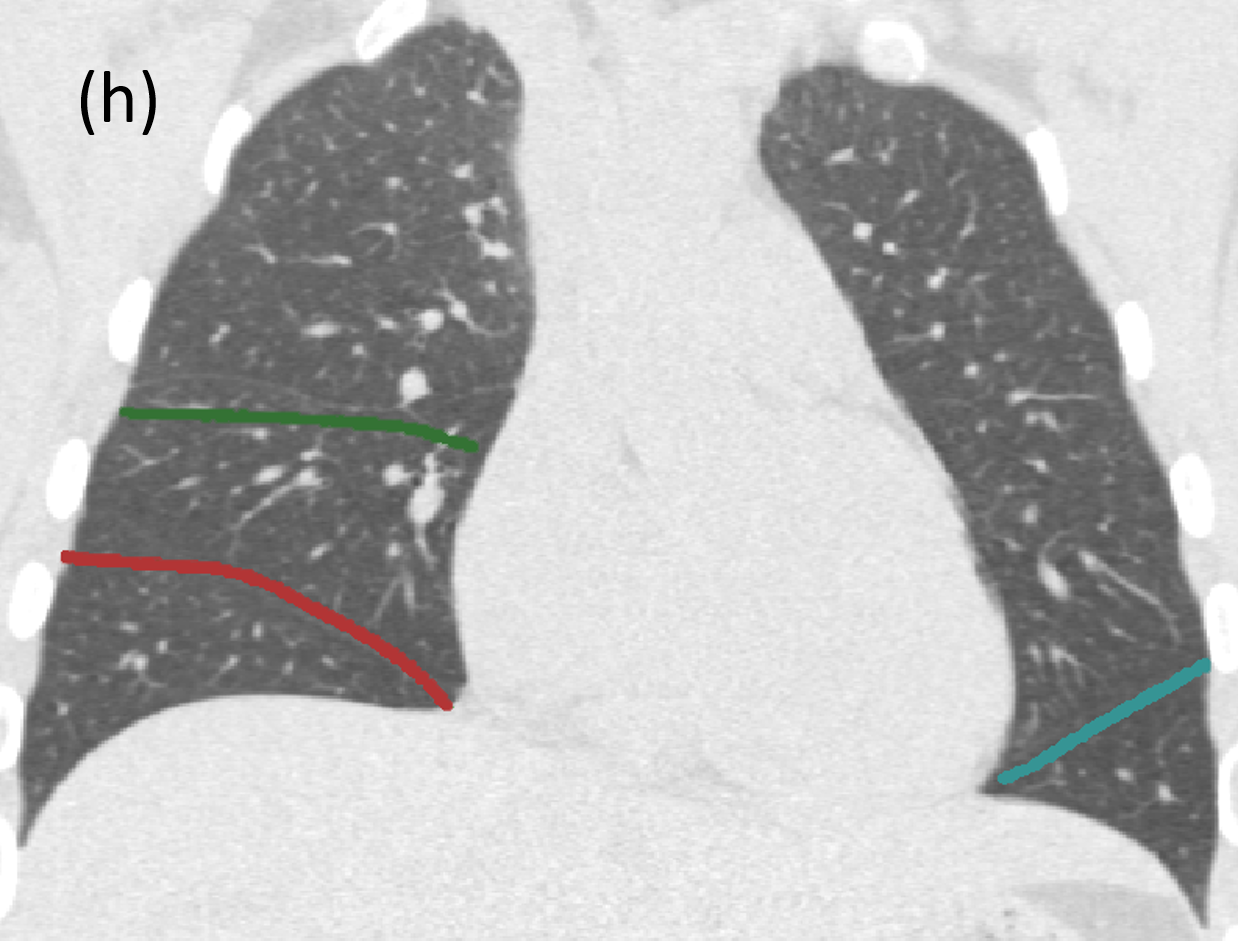
\includegraphics[width=\linewidth,trim={{.0\wd0} {.0\wd0} {.0\wd0} {.0\wd0}},clip]{Image/H1335_FRC_PCAInitial_Coronal.png}
  \centerline{}
	\end{minipage}%
   }%
  \label{fig:HLASegmentationResults-h} 
\end{subfigure}
%\vspace{.1in} % control space between the upper context and figure
%\hspace{.3in} % control space between two figures
\begin{subfigure}{
  \begin{minipage}[t]{0.2\linewidth}
  \sbox0{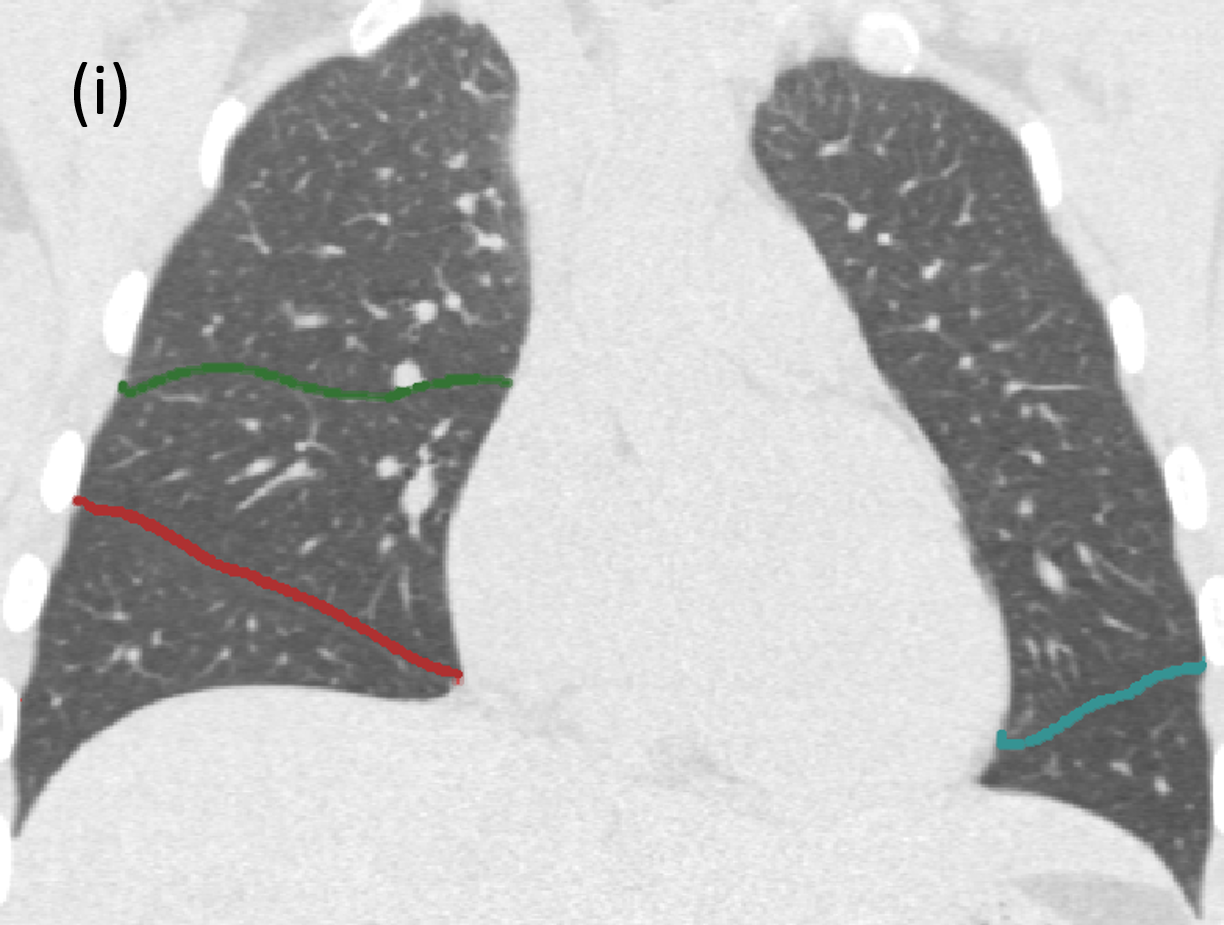
\includegraphics{Image/H1335_FRC_PCAFissureDetection_Coronal.png}}
  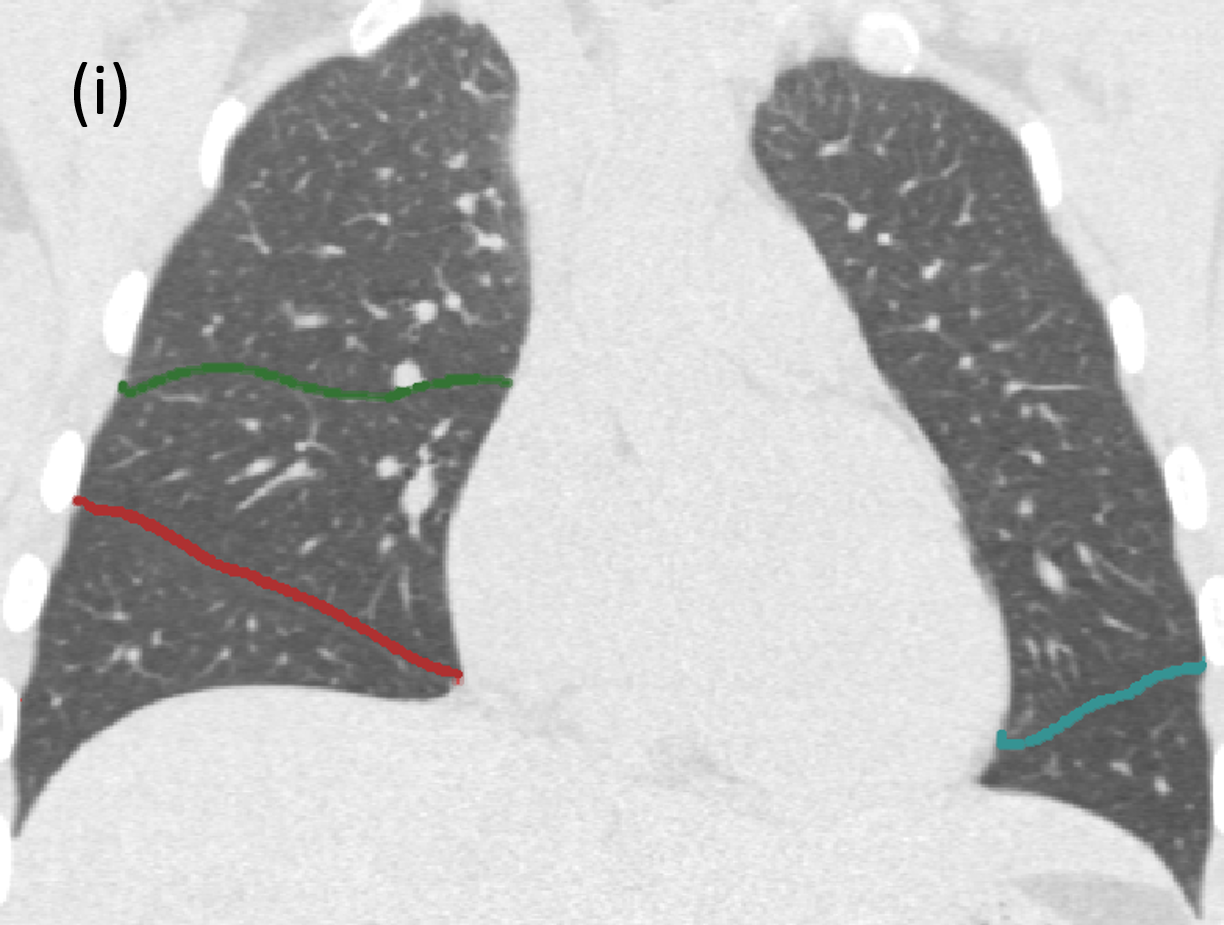
\includegraphics[width=\linewidth,trim={{.0\wd0} {.0\wd0} {.0\wd0} {.0\wd0}},clip]{Image/H1335_FRC_PCAFissureDetection_Coronal.png}
  \centerline{}
	\end{minipage}%
   }%
  \label{fig:HLASegmentationResults-i} 
\end{subfigure}
\caption{Sagittal, axial, and coronal views illustrating raw image, SSM based initial fissure guessing and final automatic fissure detection results of a normal healthy subject. (a), (d), (g) are sagittal, axial and coronal raw images. (b), (e), (h) are sagittal, axial and coronal SSM based initial fissure guessing results. (c), (f), (i) are sagittal, axial and coronal automatic fissure detection results.}
\label{fig:HLASegmentationResults}
\end{figure}

To allow for a quantitative evaluation of the performance in a healthy normal dataset and an IPF dataset, the automatic segmentation results were compared with ''gold-standard'' manual segmentations of the fissures. The ''gold-standard'' segmentations were acquired by an experienced researcher manually tracing all the three fissures for each subject by digitizing a series of points. Segmentation accuracy was quantitatively evaluated by computing the mean difference and percentage of fissure points $<$ 3 mm between the gold-standard and automatic method. The 3 mm criterion approximates the thickness of CT images routinely used clinically \cite{wei2009segmentation}. The segmentation accuracy of quantitative evaluation for normal and IPF subjects is shown in Table \ref{tab:QuantitativeResult}).

\begin{table}[htbp]
\centering
\caption{Mean error and percentile accuracy of normal healthy and IPF subjects (mean value $\pm$ standard deviation).}
\label{tab:QuantitativeResult}
\begin{tabular}{| c | c | c | c | c |}
\hline
~ & \multicolumn{2}{|c|}{\bf{Normal healthy subjects}} & \multicolumn{2}{|c|}{\bf{IPF subjects}}\\ 
\hline
~ & Mean error (mm) & Accurancy (\%) & Mean error (mm) & Accurancy (\%)\\	
\hline
Left oblique & 1.76 $\pm$ 0.68 & 81.19 $\pm$ 6.61 & 2.82 $\pm$ 0.71 & 70.26 $\pm$ 9.10\\
\hline
Right horizontal & 3.66 $\pm$ 1.37 & 64.81 $\pm$ 13.19 & 5.39 $\pm$ 1.90 & 58.43 $\pm$ 14.53\\
\hline
Right oblique & 2.55 $\pm$ 0.90 & 73.81 $\pm$ 7.96 & 4.71 $\pm$ 1.60 & 62.86 $\pm$ 11.21\\						
\hline
\end{tabular}
\end{table}

Figure \ref{fig:QuanlititativeResult} shows the spatial distribution of error for three representative subjects. Error was highest in regions close to the hilum (where the anatomical structures are complex, and/or the fissure is often incomplete on CT), and where the right fissures meet. 

To investigate the contribution of using the approximated lobe borders from the deformation of SSM, here the method is compared to two interactive watershed-based pulmonary lobe segmentation softwares: 1. Pulmonary Toolkit, PTK, https://github.com/tomdoel/pulmonarytoolkit; 2. Pulmonary Analysis Software Suite, PASS \cite{guo2008pulmonary}. Both of these softwares have a built-in lobe segmentation method which is guided by vessel tree and airway tree. The two segmentation softwares PASS and PTK tested for comparison were unable to segment the lobes for 9/20 and 7/20 subjects respectively (1/10 and 1/10 normal and 8/10 and 6/10 IPF subjects). In contrast, the model-based method gave an initial estimate for all subjects at all volumes. The main reason for the failure of segmentation is that the airway trees can't be segmented or labelled as lobar branches correctly.

\begin{figure}[htbp] 
\centering
\begin{subfigure}{
  \begin{minipage}[t]{0.21\linewidth}
  \sbox0{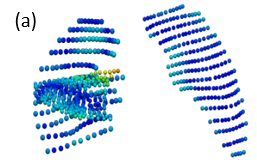
\includegraphics{Image/QuanlititativeResult1.png}} 
  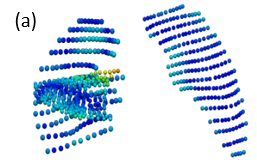
\includegraphics[width=\linewidth,trim={{.0\wd0} {.0\wd0} {.0\wd0} {.0\wd0}},clip]{Image/QuanlititativeResult1.png} %trim={<left> <lower> <right> <upper>}, set the cut scale
  \centerline{}
	\end{minipage}%
   }%
  \label{fig:QuanlititativeResult-a} 
\end{subfigure} 
\begin{subfigure}{
  \begin{minipage}[t]{0.19\linewidth}
  \sbox0{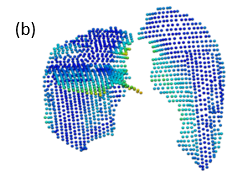
\includegraphics{Image/QuanlititativeResult2.png}}
  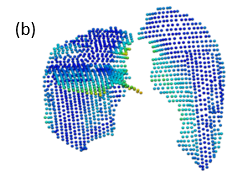
\includegraphics[width=\linewidth,trim={{.0\wd0} {.0\wd0} {.0\wd0} {.0\wd0}},clip]{Image/QuanlititativeResult2.png}
  \centerline{}
	\end{minipage}%
   }%
  \label{fig:QuanlititativeResult-b} 
\end{subfigure}
\begin{subfigure}{
  \begin{minipage}[t]{0.24\linewidth}
  \sbox0{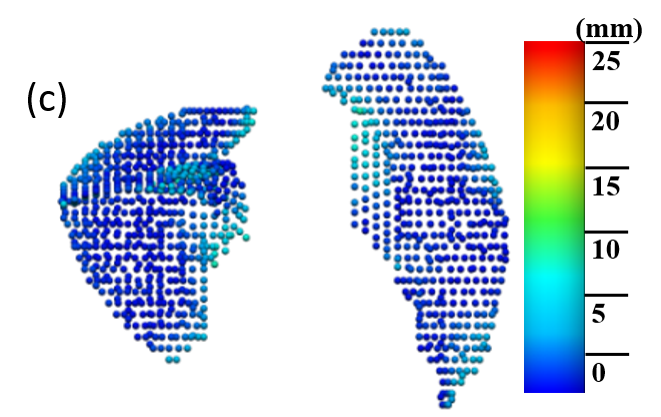
\includegraphics{Image/QuanlititativeResult3.png}}
  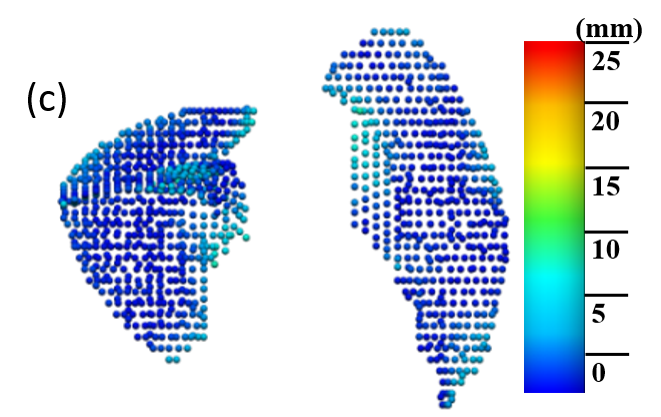
\includegraphics[width=\linewidth,trim={{.0\wd0} {.0\wd0} {.0\wd0} {.0\wd0}},clip]{Image/QuanlititativeResult3.png}
  \centerline{}
	\end{minipage}%
   }%
  \label{fig:QuanlititativeResult-c} 
\end{subfigure}
\caption{The spatial distribution of error between the gold-standard and semi-automatic methods for three representative subjects, highlighting localized regions of low accuracy.}
\label{fig:QuanlititativeResult}
\end{figure}


\section{DISCUSSION AND CONCULSION}
In this paper, a novel SSM-based pulmonary lobar segmentation method was presented and compared against two existing softwares (PTK and PASS). Results show that the method outperforms both PTK and PASS, perform well to detect the location of the fissures over most of the fissure surfaces on CT images from normal subjects, and provides a relatively accurate result for most of the IPF (abnormal) subjects. Due to lower imaging resolution and tissue abnormalities, the accuracy of the method was lower for the IPF subjects than the healthy subjects. However, the method was able to detect a fissure in each case, whereas existing research-focussed software can not, especially for the abnormal subjects. Automated segmentation of anatomical structures is still challenging in cases with abnormalities, however, the method did not fail, and it provides a robust basis for segmentation even in abnormal cohorts.

The new SSM-based method performed better on the left oblique fissure than the other two fissures, likely because the left lung has a simpler anatomic structure with only one fissure. In contrast, error detection happens more often in the area of the right lung where the two fissures come into contact. This is illustrated in Figure \ref{fig:QuanlititativeResult}, which shows the error distribution over the three fissures for three subjects. It can be seen that the method results in higher error in the lung boundary area, since the fissures here are commonly incomplete on CT scans, thus few fissure candidate points can be detected accurately. There is also a high error around the junction area of the right oblique fissure and right horizontal fissure, since the two fissures are too closed in this region and the search regions may overlap with each other.

In the new method, a SSM was used to provide an initial fissure estimate. Compared to the current published anatomical structure-based methods (PTK and PASS), the SSM-based method can predict the fissure location without requiring a preliminary analysis of other anatomical features other than lung shape. For example, traditional anatomical knowledge-based methods such as the watershed-based lobar segmentation relies on the success of the automatic segmentations of the vessel and airway tree and need to label the airway trees to the five main lobar bronchi to get an initial fissure approximation. When one of those segmentations fails, the method is likely to perform worse. Vessels are distributed all over the lung and due to the high contrast to the lung parenchyma, a good segmentation of the vessels is feasible.  But in some cases vessels cross the lobar boundaries. Thus, the assumption that there are no vessels at the lobar boundary is not always correct. Due to the complex radiological appearance of pathological lungs, it is usually difficult to get a reliable airway and vessel tree segmentation. In contrast, the new method is largely independent of the knowledge of lung anatomy, so in the comparison of the SSM-based estimation of fissure location with a watershed-based method, the latter failed for nearly half of the subjects. 
%
%
%\acknowledgments % equivalent to \section*{ACKNOWLEDGMENTS}       
 %
%This unnumbered section is used to identify those who have aided the authors in understanding or accomplishing the work presented and to acknowledge sources of funding.  

% References
\bibliography{report} % bibliography data in report.bib
\bibliographystyle{spiebib} % makes bibtex use spiebib.bst

\end{document} 
